%%%%%%%%%%%%%%%%%%%%%%%%%%%%%%%%%%%%%%%%%%%%%%%%%%%%%%%%%%
%
% Vzor pro sazbu kvalifikační práce
%
% Západočeská univerzita v Plzni
% Fakulta aplikovaných věd
% Katedra informatiky a výpočetní techniky
%
% Petr Lobaz, lobaz@kiv.zcu.cz, 2016/03/14
%
%%%%%%%%%%%%%%%%%%%%%%%%%%%%%%%%%%%%%%%%%%%%%%%%%%%%%%%%%%

% Možné jazyky práce: czech, english
% Možné typy práce: BP (bakalářská), DP (diplomová)
\documentclass[czech,DP]{thesiskiv}

% Definujte údaje pro vstupní strany
%
% Jméno a příjmení; kvůli textu prohlášení určete, 
% zda jde o mužské, nebo ženské jméno.
\author{Kateřina Kratochvílová}
\declarationfemale

%alternativa: 
%\declarationfemale

% Název práce
\title{Nástroj pro automatickou identifikaci KIR alel}

\thanktext{Ráda bych poděkovala Ing. Lucii Houdové, Ph.D. za cenné rady, věcné připomínky, trpělivost a ochotu, kterou mi v průběhu zpracování této práce věnovala.}
% 
% Texty abstraktů (anglicky, česky)
%
\abstracttexten{The text of the abstract (in English). It contains the English translation of the thesis title and a short description of the thesis.}

\abstracttextcz{Text abstraktu (česky). Obsahuje krátkou anotaci (cca 10 řádek) v češtině. Budete ji potřebovat i při vyplňování údajů o bakalářské práci ve STAGu. Český i anglický abstrakt by měly být na stejné stránce a měly by si obsahem co možná nejvíce odpovídat (samozřejmě není možný doslovný překlad!).
}

% Na titulní stranu a do textu prohlášení se automaticky vkládá 
% aktuální rok, resp. datum. Můžete je změnit:
%\titlepageyear{2016}
%\declarationdate{1. března 2016}

% Ve zvláštních případech je možné ovlivnit i ostatní texty:
%
%\university{Západočeská univerzita v Plzni}
%\faculty{Fakulta aplikovaných věd}
%\department{Katedra informatiky a výpočetní techniky}
%\subject{Bakalářská práce}
%\titlepagetown{Plzeň}
%\declarationtown{Plzni}

%%%%%%%%%%%%%%%%%%%%%%%%%%%%%%%%%%%%%%%%%%%%%%%%%%%%%%%%%%
%
% DODATEČNÉ BALÍČKY PRO SAZBU
% Jejich užívání či neužívání záleží na libovůli autora 
% práce
%
%%%%%%%%%%%%%%%%%%%%%%%%%%%%%%%%%%%%%%%%%%%%%%%%%%%%%%%%%%

% Zařadit literaturu do obsahu
\usepackage[nottoc,notlot,notlof]{tocbibind}

% Umožňuje vkládání obrázků
\usepackage[pdftex]{graphicx}

% Odkazy v PDF jsou aktivní; navíc se automaticky vkládá
% balíček 'url', který umožňuje např. dělení slov
% uvnitř URL
\usepackage[pdftex]{hyperref}
\hypersetup{colorlinks=true,
  unicode=true,
  linkcolor=black,
  citecolor=black,
  urlcolor=black,
  bookmarksopen=true}

% matematicke rovnice %
\usepackage{amsmath}
\usepackage{fancyhdr}
\usepackage{float}
\numberwithin{equation}{section}
% Při používání citačního stylu csplainnatkiv
% (odvozen z csplainnat, http://repo.or.cz/w/csplainnat.git)
% lze snadno modifikovat vzhled citací v textu
\usepackage[numbers,sort&compress]{natbib}

%%%%%%%%%%%%%%%%%%%%%%%%%%%%%%%%%%%%%%%%%%%%%%%%%%%%%%%%%%
%
% VLASTNÍ TEXT PRÁCE
%
%%%%%%%%%%%%%%%%%%%%%%%%%%%%%%%%%%%%%%%%%%%%%%%%%%%%%%%%%%
\begin{document}
%
\maketitle
\tableofcontents

\chapter{Úvod}

něco o transplantaci kostní dřeně, narazit že když by bylo 10/10 tak by bylo vhodné dělat porovnání těch KIR
něco o AML
Obtížnost transplantace krvetvorných buněk nespočívá v lékařské části procesu,
nýbrž v následné imunitní odpovědi organismu.
Proč KIR? pOrotože roste počet důkazů vluvu genů KIR že mají vliv na výsledky transplance  při leukemii
NK buňky byli identifikovány jako schopné zabíjet nádorové buňky bez omezení lidského leukocytového antigenu (HLA)
Oproti T-lymfocitům který potřebují HLA molekulu ke zprostředkování jejich činností
NK odpovídají také na virové infekce v časné fázi ale bohužel i do odmítnutí transplantace orgánů či buněčné
Z toho jak jsem tam našla tu velkou buňku


\chapter{Imunitní systém a jeho spojitost s geny}
\section{Geny}
V každé buňce lidského organismu, konkrétně v buněčném jádře, je možné nálest 46 chromozomů. Jeden chromozom představuje stočenou dlouhou molekulu DNA (Deoxyribonuklenovou kyselinu). Všech 46 chromozomů obsahuje okolo 100 000 genů. Drobný segment DNA, který řídí buněčnou funkci je právě gen. Konkrétní forma genu je alela. \citep{en_smith}

\begin{figure}[H]		
		\centering
		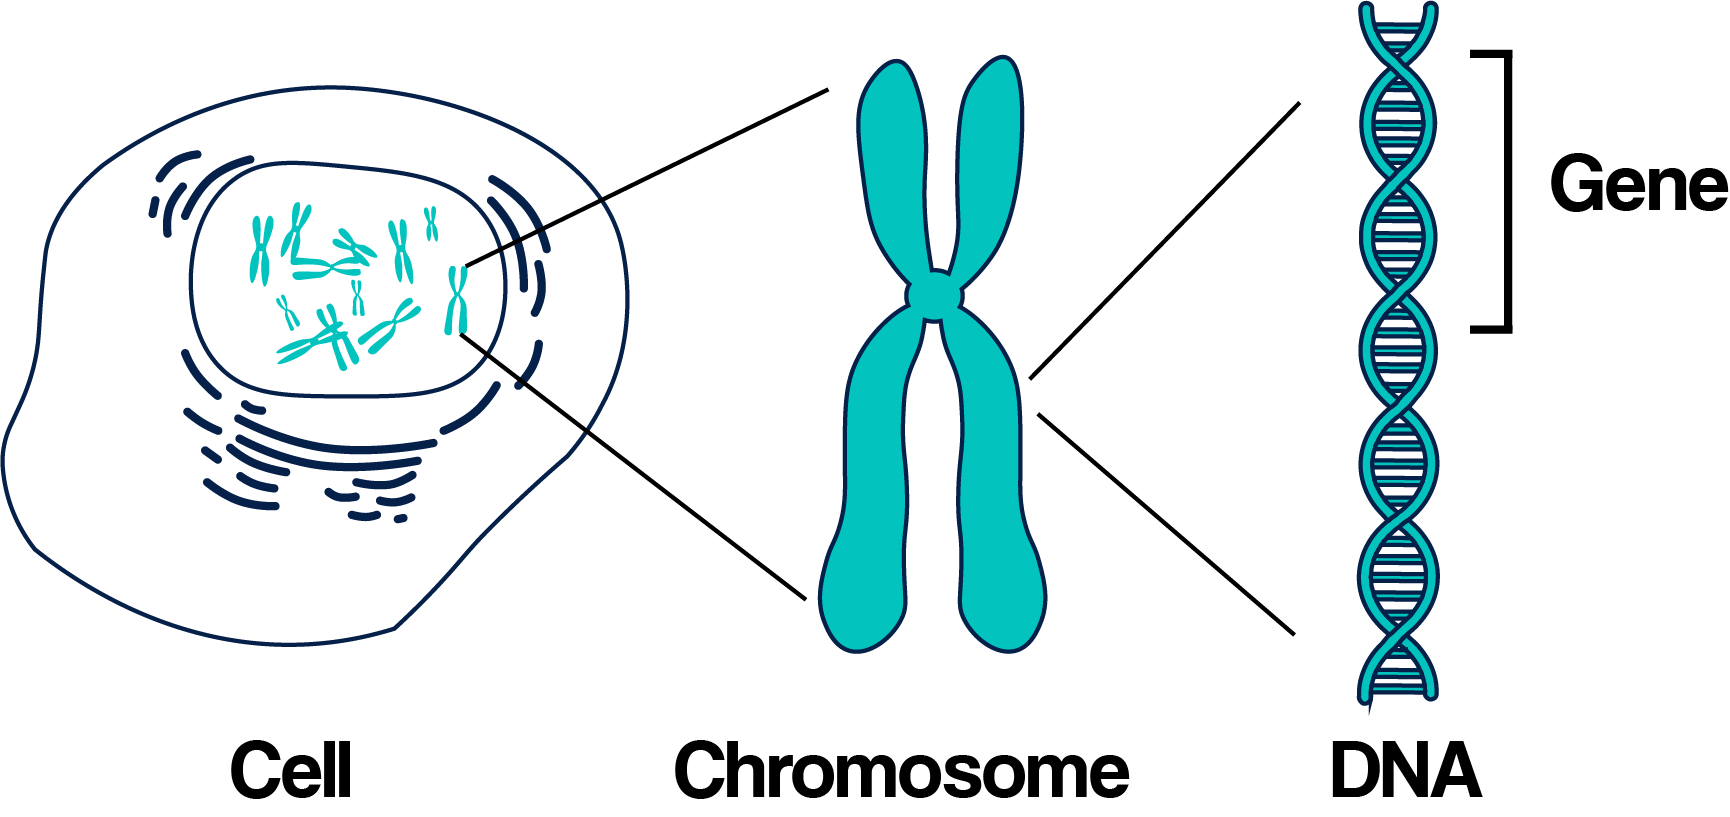
\includegraphics[width=200px]{./img/lidska_bunka.png}
		\caption{Gen a vztah k lidské buňce. \cite{human_cell}}
		\label{fig:bunka_gen}
\end{figure}

\begin{figure}[H]		
		\centering
		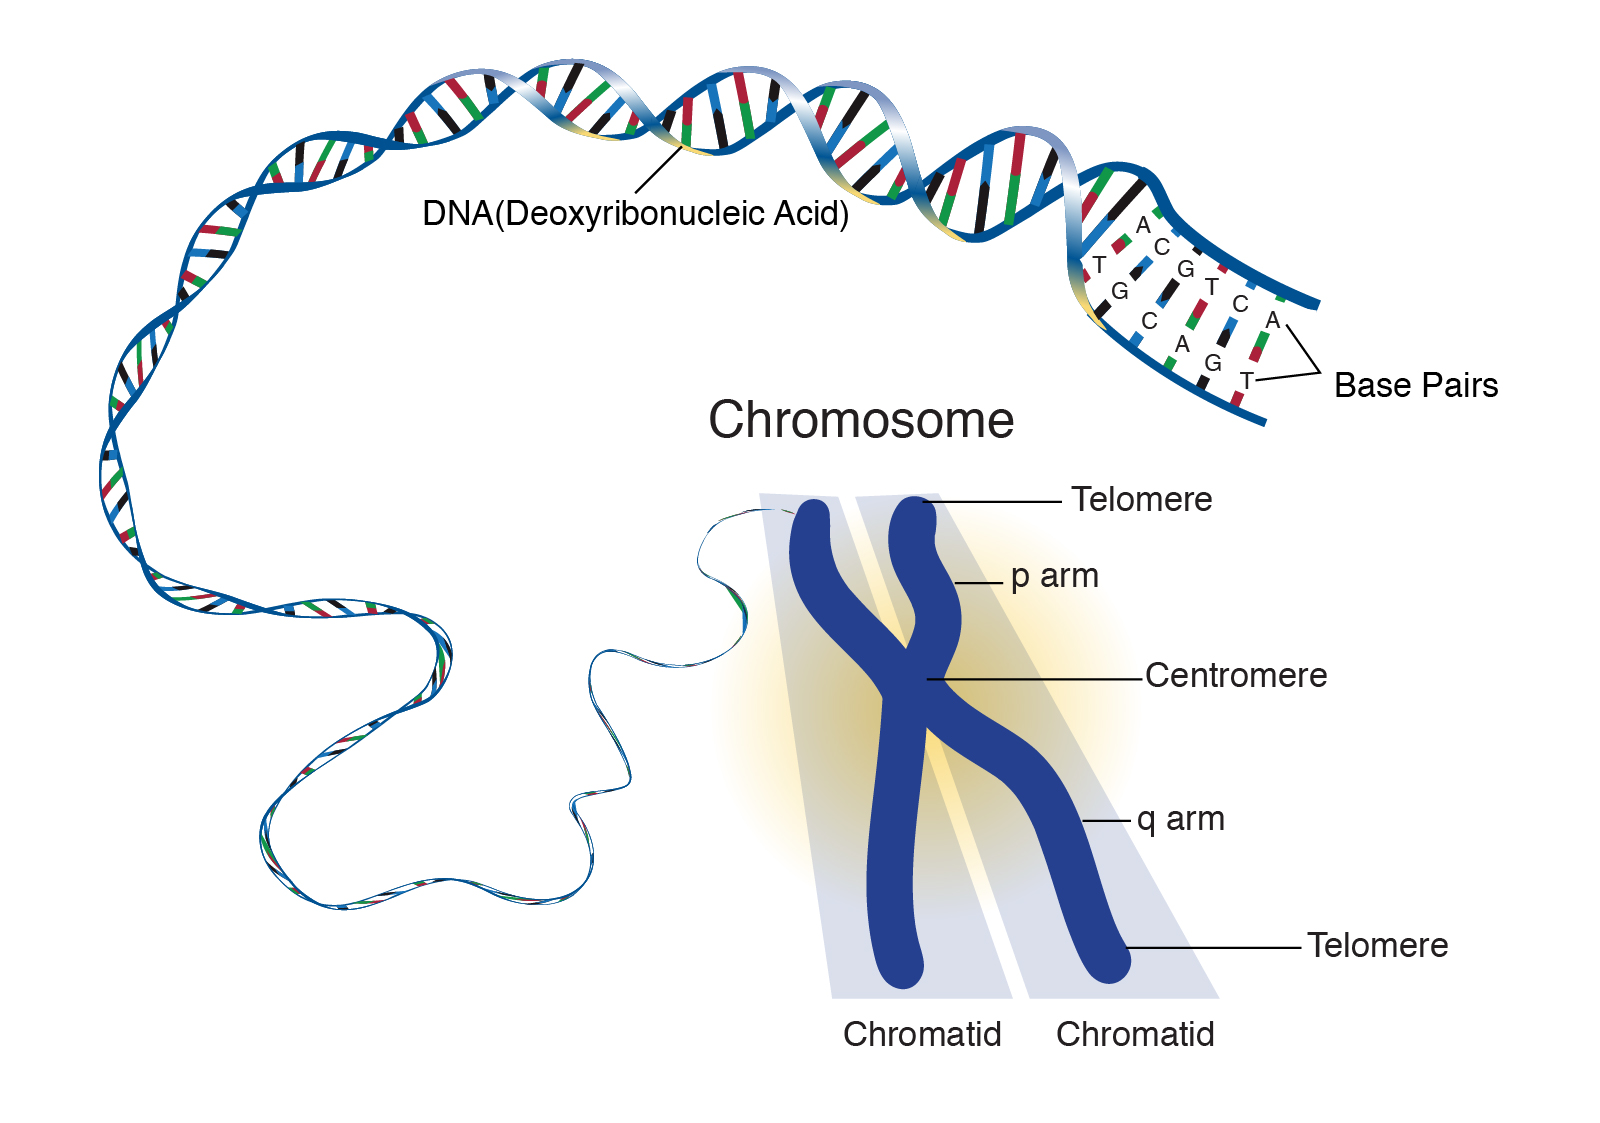
\includegraphics[width=250px]{./img/chromosome.jpg}
		\caption{Struktura chromozomu. Na tomto obrázku je důležité si povšimnout p a q raménka a centromeru. \cite{chromosome_structure}}
		\label{fig:chrmosome}
\end{figure}

Uvnitř buňky máme celý genom který se ovšem nemusí projevit na povrchu buňky. Pokud se vlastnost kterou gen přenáší projeví na povrchu buňky označujeme to jako exprese genu (jeho sebevyjádření). Od toho se odvíjí i označování něco za KIR gen či KIR receptor nebo molekulu.


\section{Imunitní systém}
Imunitní systém chrání organismus před škodlivinami. Skládá se ze dvou hlavních částí vrozené imunity a získané imunity. 

\subsection{Vrozená imunita}
Vrozená imunita též označována přirozená, neadaptivní, antigenně nespecifická je neměnně zapsána v DNA. To znamená, že při každém setkání s antigenem odpoví stejnou reakcí. Buňky nesoucí vrozenou imunitu jsou stále přítomně v krvy, takže jejich případná aktivace je takřka okamžitá (minuty až hodiny). Do této imunity patří i natural killer buňky s KIR receptory, které budou dále rozebírány v textu. 

\subsection{Získaná imunita}
Získaná imunita též označována specifická či adaptivní oproti specifické má v genomu zapsány pouze své základy. V průběhu lidského života se vyvyjí a mění. Změna může nastat například očkování nebo proděláním patřičné choroby. Tato změna ovšem nemusí být trvalá. Z těchto důvodů může být odpověď ziskáné imunity při setkání se stejnou chorobou rozdílná. Fungování získané imunity zajišťují T- a B- lymfocyty, ale nefunguje samostantně. Při zabíjení patogenů spolupracuje s vrozenou imunitou.

\subsection{Antigen}
Antigeny jsou látky, které imunitní systém rozpozná a zareaguje na ně. V podstatě to může být jakákoli bílkoviná sloučenina. Antigen se obvykle nachází na povrchu buňky jako vyjádření genu. Imunitní systém následně zjistí o jaký antigen se jedná, respektivě o jakou buňku se jedná, zda tělu vlastní (např. zdravá buňka) nebo buňku tělu cizí (např. nádorová buňka), tedy jedná-li se o expresy lidského genu nebo například viru. Jedná-li se o buňku tělu cizí imunitní systém reaguje snahou ji zničit.


\section{HLA a non-HLA geny}
Human leucocyte antigen (HLA) je genetický systém, který je primárně zodpovědný za rozeznávání vlastního od cizorodého. Někdy je termín HLA zaměňován s MHC. MHC (Major histocompatibility complex) je souhrný termín pro všechny komplexy, kdy podskupinou jsou práve HLA (H - Human) který je pro lidi. Stejně tak existuje DLA (D - Dog) který je pro psy. Z funkčního i biologického hlediska jde však u všech savců o stejnou skupinu genů. \cite{KIR_transplantace_jindra}
\\
\\
HLA a některé non-HLA geny se nacházejí na krátkém raménku 6 chromozomu, konkrétně 6p21.3 a zaujímá úsek přibližně jednu tisícinu genomu. Tento region je nejvíce komplexní a polymorfní na lidském genomu s více než 220 geny. Oproti tomu jedna ze skupin non-HLA genů, konkrétně KIR geny, se nachází na 19 chromozomu. Rozsáhlá diverzita genů vznikala snahou eliminovat neustále se měnící spektrum patogenů. Produkty těchto genů na povrch buňky významně ovlivňují odpověď na infekční choroby a výsledky buněčné či orgánové transplantace. \cite{imgt_hla_database}


\begin{figure}[H]		
		\centering
		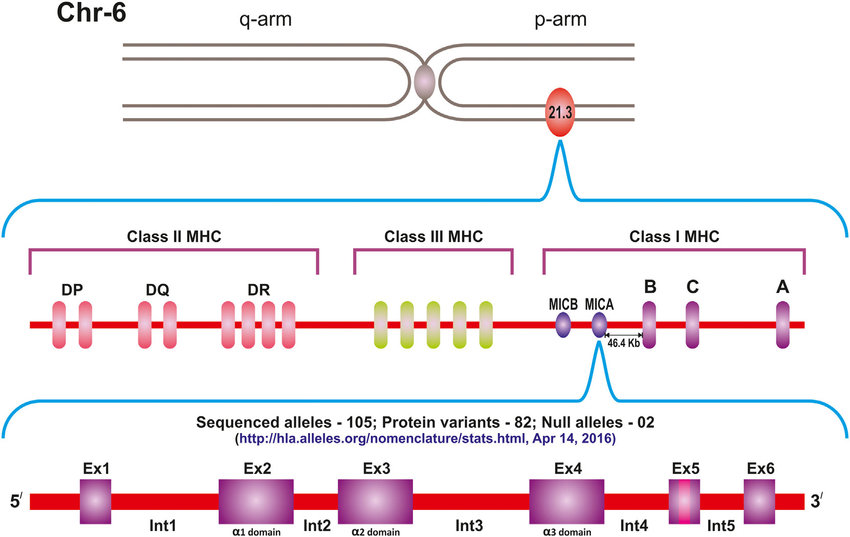
\includegraphics[width=300px]{./img/genom6_mica.jpg}
		\caption{6 chromozom. TODO ten spodní řádek bych asi usekla- stejně nevím co to znamená. }
		\label{fig:hla_genome}
\end{figure}

\noindent
Přesná definice mezi HLA a non-HLA geny neexistuje. Mimo jiné i jejich rozdělení není v literaturách sjednocené. Jak je vidět z obrázku \ref{fig:hla_genome} je možné geny rozdělit do tří tříd. V některých literaturach je možné nalést označení non-HLA genů jako geny III.třídy v jiné, že jsou to všechny geny III třídy a některé geny třídy I. Tato práce se bude v označení za gen non-HLA či HLA odkazovat na hla.alleles \cite{imgt_hla_database}. Zjednodušeně tedy můžeme říci, že geny které nejsou řazeny k HLA skupinám jsou non-HLA. Je-li gen označen za non-HLA neznamená to, že by neměl souvislost s funkcí imunitního systému. Naopak má, jen ne výlučně s HLA systémem. Non-HLA geny kódují produkty spojené s imunitními procesy. Mezi non-HLA geny mimo jiné patří MICA, MICB a KIR. \cite{imgt_hla_database}

\section{Natural killer a jeho receptory}
\subsection{Natural killer}
Natural killer buňky (NK buňky) jsou velké granulární lymfocyty vrozeného imunitního systému. V krevním oběhu lidského těla je jich možné nalést $10-15\%$. Klíčovou vlastností NK buněk je nejenom schopnost rozlišit poškozené buňky od zdravích, ale i poškozené buňky rychle a efektivně likvidovat. Poškozené buňky mohou být buňky infokované virem či buňky transfomované v nádorové. Na povrchu NK buňky se nachází receptory, které jsou zobrazeny na obrázku \ref{fig:NK_receptors}, regulující odpověď imunitního systému. Natural killer buňky oproti B- a T- lymfocitům (buňkám získané imunity) nemají antigenně specifické receptory. Jedním ze způsobům jak NK buňky rozpoznávají a zabíjejí poškozené buňky je na základě interakce mezi KIR receptorem a HLA molekulou na povrchu zkoumané buňky. Stejně tak mohou zabíjet na základě receptoru NKG2D, který aktivuje cytoxickou reakci při setkání s ligandem MICA a MICB.
 

\begin{figure}[H]		
		\centering
		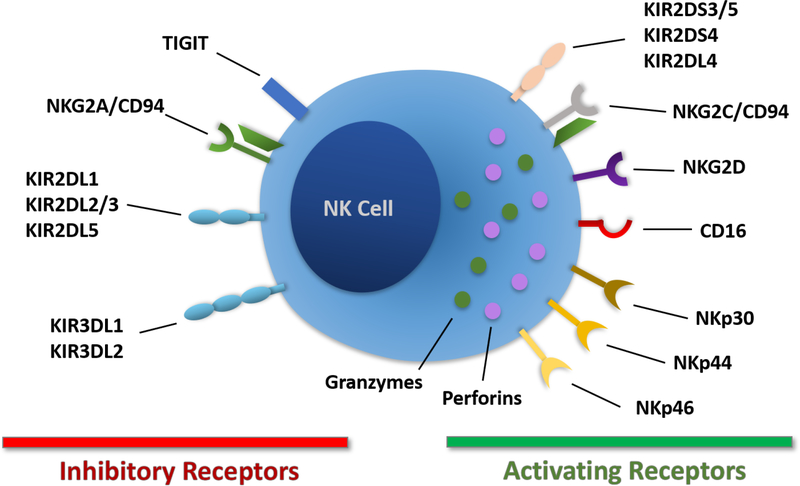
\includegraphics[width=300px]{./img/nk_receptory.jpg}
		\caption{Natural killer buňka a její receptory, rozděleny na aktivační a inhibiční. Pro tuto práci jsou důležité hlavně KIR receptory a NKG2D. \cite{NK_receptors} }
		\label{fig:NK_receptors}
\end{figure}

\subsubsection{Ligand}
Ligandem označujeme malou molekulu, která se váže na vazebné místo cílového proteinu a vyvolává fyziologickou odpověď. 
TODO - wikipedie!!!!


\subsection{Receptor NKG2D a jeho ligandy MICA/MICB}
NKG2D je receptor na NK buňce rozpoznávající především buněčný stres a může spustit cytotoxicitu (shopnost níčit buňky) i když se na povrchu buňky nachází inhibiční HLA-I ligandy.  
\\
\\
Geny skupiny MICA a MICB jsou dle hla.alleles \cite{imgt_hla_database} označeny jako class I chain-related gene. To znamená, že se běžně neřadí do I. třídy. Oproti HLA genům, které mají svoje produkty na lymfocytech, se produkty MICA a MICB nachází na epitelových buňkách. Nejedná se tedy o standardní HLA geny, proto jsou nověji v literaturách označovány jako non-HLA. Jejich expresí na povrch buňky jsou ligandy, které se váží na receptor NKG2D. Buňky s ligandy MICA a MICB se množí při nádorovém onemocnění, zanětu nebo pod vlivem různých forem buněčného stresu a díky navázáním na receptor může být spuštěna imunitní reakce. \cite{transfuzni_lekarstvi} \cite{MIC} \cite{NK_receptors}


\subsection{KIR}
Killer immunoglobulin-like receptor (KIR) je skupina genů řazených mezi non-HLA geny. Jejich zvláštností je fakt, že se nenachází na 6 chromozomu, ale na 19 a tak shodní dárci HLA znaků mohou být neshodní v KIR znacích. Jejich expresí jsou receptory na povrchu natural killer buněk. Dnes je známo 15 genů a 2 pseudogeny rozlišujících se na inhibiční a aktivační na základě cytoplasmatického ocásku a počtu imunoglobulínových domén. \citep{KIR_transplantace_jindra}


\begin{figure}[H]		
		\centering
		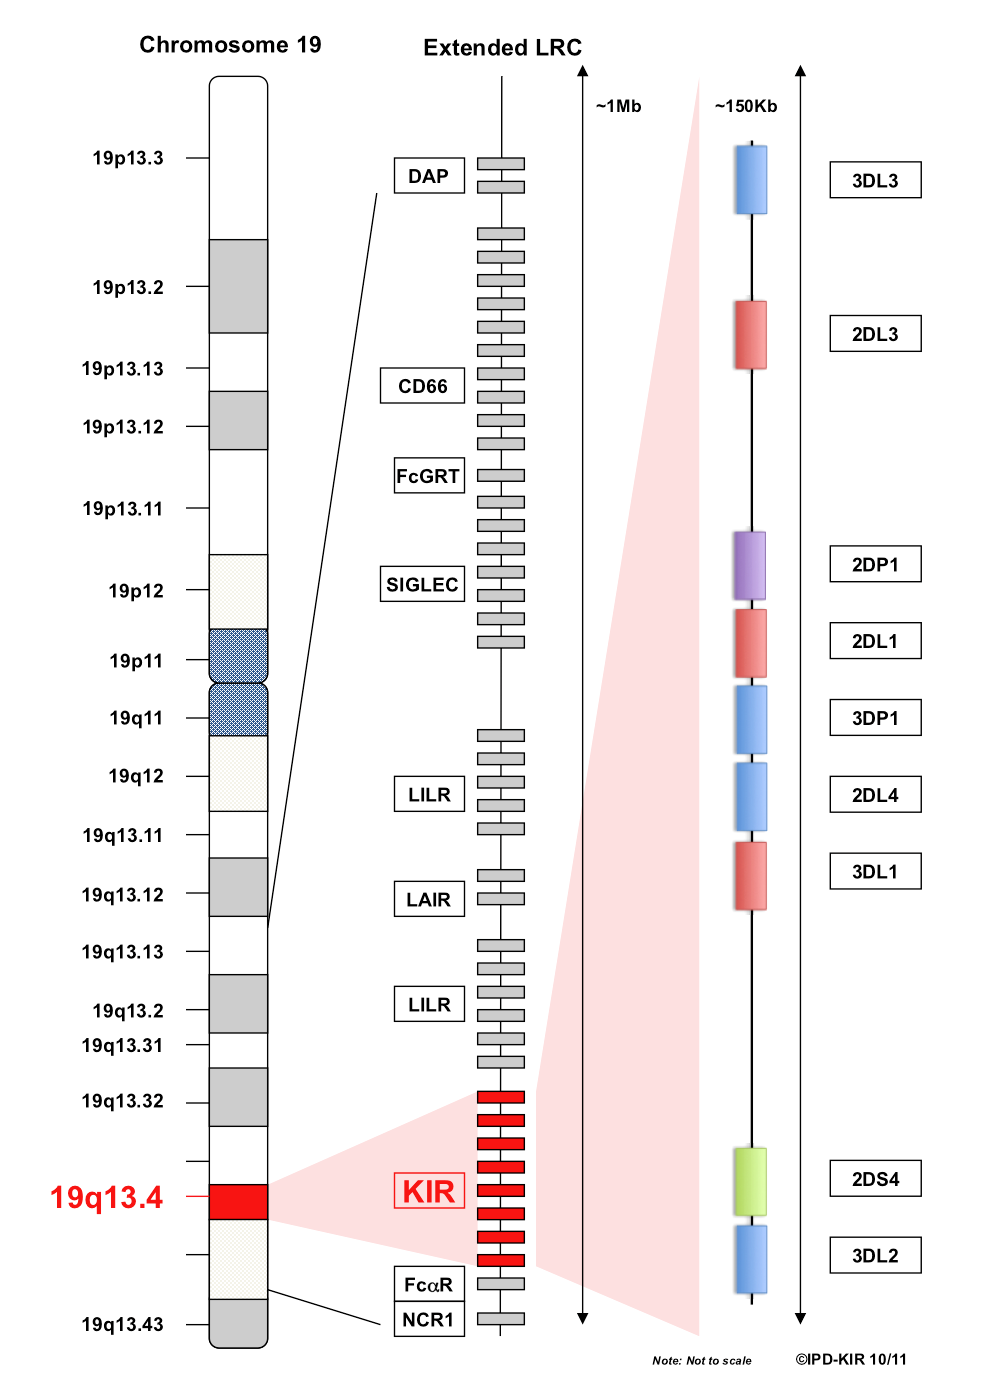
\includegraphics[width=250px]{./img/kir_pozice.png}
		\caption{KIR se nachází na 19 chromozomu v oblásni jménem leukocyte receptor complex (LRC). \cite{imgt_hla_database}}
		\label{fig:kir_position}
\end{figure}

\noindent
Jak již bylo výše zmíněno KIR receptory můžeme rozdělit na inhibiční a aktivační. Zda dojde k aktivaci NK buňky rozhoduje právě jejich rovnováha na zkoumané buňce. Zatímco inhibiční receptory se váží hlavně na molekuly HLA, aktivační receptory rozpoznávají molekuly které jsou exprimovány na membránu při buněčném stresu.
\\
\\
NK buňky ustavičně prohledávají své okolí a testují přítomnost příslušných HLA ligand (specifická HLA molekula) pro své KIR receptory. Pokud je příslušný HLA ligand přítomen naváže se na NK buňku (\ref{fig:kir_princip} případ~1). Tímto systémem jsou ochráněny vlastní HLA buňky. Pokud přítomen není je spuštěna cytotoxická reakce a zkoumaná buňka je zníčena.
\\
\\
Některé virem napadené buňky potlačují propsání HLA ligand na povrch buňky a tím se brání cytotoxicitě proti T lymfocitům, ale naopak jsou více citlivější na cytotoxicitu proti NK buňkám. Ukázano na obrázku \ref{fig:kir_princip} případ~3.
\begin{figure}[H]		
		\centering
		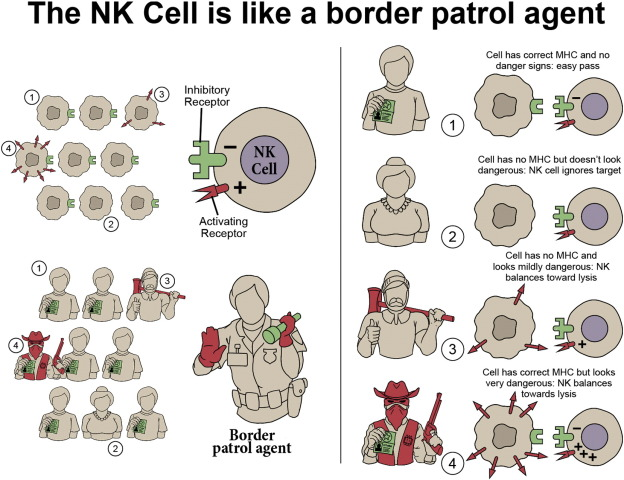
\includegraphics[width=\textwidth]{./img/NK_princip.jpg}
		\caption{Přirovnání fungování natural killer buňky k pasové kontrole \cite{KIR_img_princip}. V pravé části jsou zobrazené případy které mohou nastat když natural killer buňka potká jinou buňku. V prvním případě je tělu vlastní zdravá buňka, kde se KIR receptor naváže na HLA ligand a k cytotoxitické reakci nedojde. V druhém případě je červená krvinka k cytotoxicitě opět nedojde, protože na zkoumané buňce nepřevažují aktivační receptory. V 3 případě je to nádorová buňka, která schová HLA ligand (může nastat po transplantaci kostní dřeně) a tím se "schová" proti T- lymfocytům. Avšak aktivační receptory převládají a tak k cytotoxicitě dojde. Ve 4 příkladě je nádorová buňka nebo virem nakažená buňka (stresové ligandy). Aktivační receptory převládají k cytotoxicitě dojde.}
		\label{fig:kir_princip}
\end{figure}


\subsection{Nomenklatura KIR genů}
KIR geny (na obrázku \ref{fig:img_kir_nomenklatura}) se liší různou délkou cytoplasmatických ocásku (tail) a různým počtem imunoglobulin-like domén (lg-like). Na základě této rozmanitosti byla založena nomenklatura KIR genů, tedy jejich pojmenování. 
\\
\\
Jak je vidět na obrázku~\ref{fig:img_kir_nomenklatura}, cytoplasmatický ocásek může být dlouhý (long~-~L) nebo krátký (short~-~S). Oproti tomu imunoglubulínové domény se mohou vyskytovat 2~(2D) nebo 3~(3D). 

\begin{figure}[H]		
		\centering
		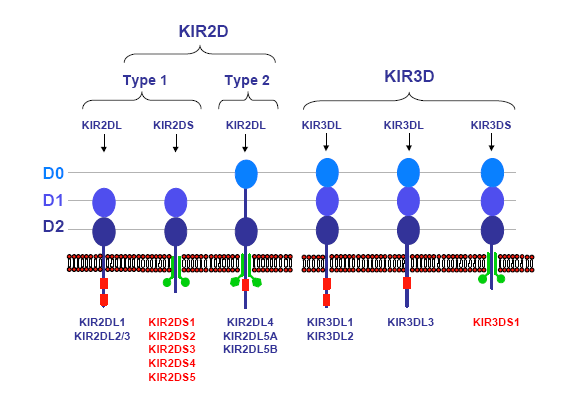
\includegraphics[width=\textwidth]{./img/KIR_nomenklatura.png}
		\caption{Nomenklatura KIR genů. \cite{KIR_transplantace_jindra}}
		\label{fig:img_kir_nomenklatura}
\end{figure}

\noindent
Další rozdělení KIR genů je již výše zmíněné inhibiční a aktivační. Na obrázku~\ref{fig:img_kir_ligand} je možné si povšimnout detailu, že až na KIR2DL4 jsou aktivační KIR s krátkým ocáskem, zatímco inhibiční jsou s dlouhým ocáskem. Obrázek dále uvádí vazebné ligandy pro jednotlivé receptory. 
 
\begin{figure}[H]		
		\centering
		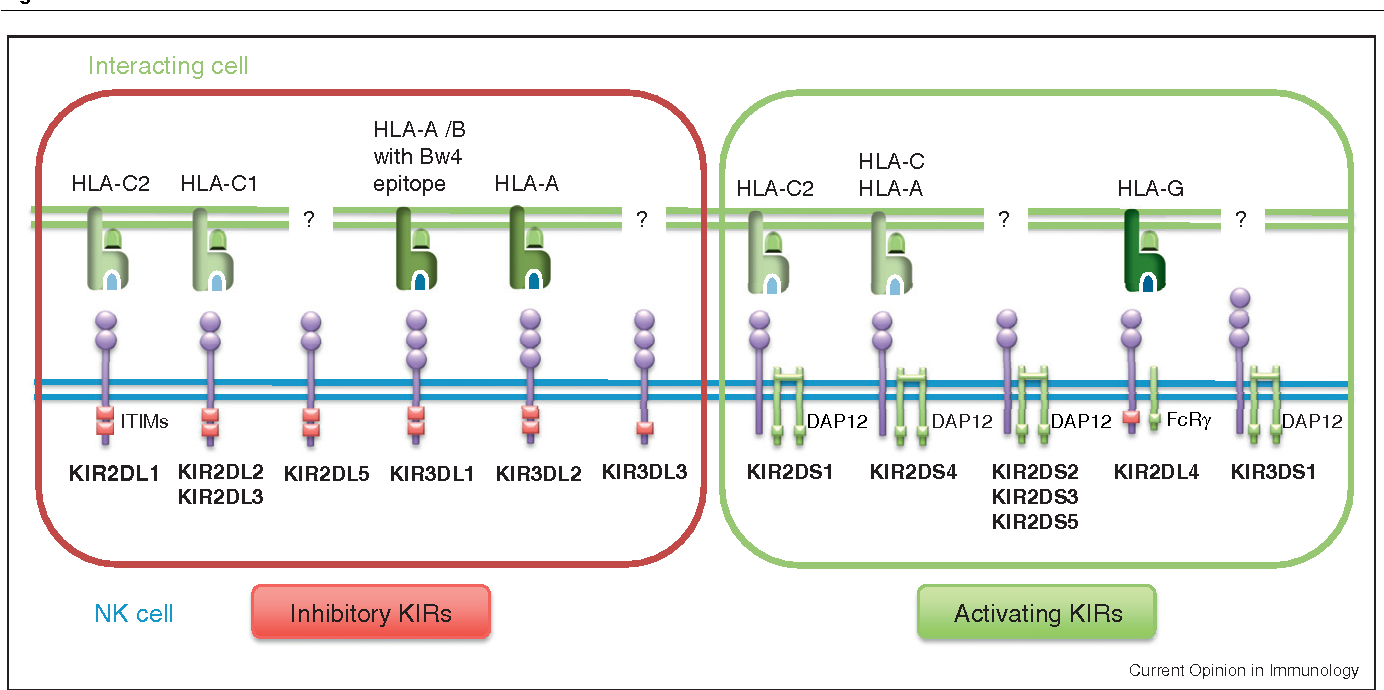
\includegraphics[width=\textwidth]{./img/KIR_nomenklatura2.png}
		\caption{KIR geny a jejich vazebné ligandy. Pokud je v obrázku ? značí to, že pro daný receptor neni znám vazebný ligand. \cite{KIR_img_nomenklatura}}
		\label{fig:img_kir_ligand}
\end{figure}

\subsection{KIR haplotyp}
KIR haplotyp je vyjádření jaké konkrétní KIR geny genom obsahuje. Doposud nebylo zavedeno konkrétní pravidlo na jejich pojmenovávání. Avšak bylo navrženo, aby každý KIR haplotyp byl označen $"KH-"$ následovaným trojmístným číslem, které bude označovat konkrétní haplotyp. Bylo by tak možné pojmenovat 999 haplotypů. 
\\
\\
Dále by se haplotypy rozdělovali na dvě skupiny A a B. Skupina B musí obsahovat alespoň jeden z genů KIR2DL5, KIR2DS1, KIR2DS2, KIR2DS3, KIR2DS5 a KIR3DS1. Naopak skupina A neobsahuje ani jeden z těchto genů. Z tohoto pravidla je patrné, že haplotypy B mají vždy více aktivačních KIR než haplotypy A. Za trojmístným číslem by tedy dále bylo písmeno A nebo B.
\\
\\
Nakonec by byl připojen 17-ti místný binární kód, který by označoval přítomnost $"1"$ či absenci $"0"$ genu. Pořadí genů by odpovídalo pořadí v genomu.
\\
\\
Výsledné pojmenování by mohlo vypadat následovně:
\begin{align}
   \label{kir_haplotyp} KH-001A-11100010011011011
\end{align}

\noindent
Je třeba si zde uvědomit, že každý jedinec má 2 KIR haplotypy. Je tedy možné dostat 4 kombinace - A/A, A/B, B/A nebo B/B. Haplotyp jedince je označován za A v případě kdy má kombinaci A/A a za B v případě jedné z kombinací A/B, B/A nebo B/B. Je možné si povšimnout, že u haplotypu A převládají inhibiční KIR geny a proto jsou dárci lépe přijímáni. Zatímco haplotyp B má převahu aktivační KIR a proto má vliv na celkové přežití.


\section{Porovnání vhodného dárce}
Mezi rizika při transplantaci krvetvorných buněk patří reakce štěpu proti hostiteli nebo relaps oněmocnění (návrat nemoci). Ač je dárce vybírán podle shody v HLA znacích, sekundární kriteria jako jsou pohlaví a věk mohou také hrát roli pro úspěšnost transplantace. Navíc podle nedávných studiích výsledky příjetí štěpu ovlivňují nejenom HLA geny ale i non-HLA geny. Jedním z nich může být právě killer immunoglobulin-like receptor (KIR). V případě kdy by bylo nalezeno více vhodných dárců, tj. se shodou 10/10 nebo 9/10, vybíralo by se následně podle KIR genů. \cite{KIR_transplantace_jindra} \cite{Frycova_bakalarka}
\\
\\
Při určování shody dárce a pacienta se rozhoduje na základě schody alel u genů HLA -A, -B, -C, -DRB1, -DQB1. Díky velké diverzitě HLA genů je počet možných kombinací několik miliard. Některé kombinace genů se vyskytují na základě oblasti či národnosti častěji nebo mohou být naopak vzácné. HLA geny se obvykle dědí jako blok (cely haplotyp), avšak ve výjmečných případech může dojít k rekombinaci. Z tohoto důvodu je nejsnadnější nalést shodu v pokrevním příbuzenstvu.
\\
\\
Jelikož každý jedinec má dvakrát geny na pozicích HLA -A, -B, -C, -DRB1 a -DQB1 (jednu pětici od otce, druhou pětici od matky), je maximální shoda 10/10 (shoda obou alel v lokusech). Čím je shoda menší tím větší je riziko nepřijetí stěpu. U nepříbuzných jedinců lze tolerovat shodu 9/10 či 8/10. \cite{Frycova_bakalarka} \cite{KIR_transplantace_jindra}
\\
\\
V posledních letech se objevuje Haploidentická transplantace, kdy je možné použít krvetvorné buňky příbuzného pouze s poloviční shodou (např. všichni rodiče a děti). Umožnuje to podávání chemoterapie pár dní po transplantaci, která zníčí všechny buňky, které tělo nepřijme. Využívá se toho hlavně v případech časové tísně, kdy není čas hledat dárce v registrech. \cite{haploidenticka_transplantace}
\\
\\
KIR geny se stejně jako HLA dědí celý blok. Jelikož HLA se nachází na 6 chromozomu a KIR na 19, tak shodní dárci v HLA znacích se jen menšinově shodují v KIR genech. V případě příbuzného dárce shodujícího se v HLA znacích je pouze 25\% shodných také v KIR. \cite{KIR_haplotypy}
\\
\\
K zjištění typizace se používají sekvenační metody, typicky s polymerázovou řetězovou reakcí. 


\section{Bordel haplotypy}
TODO centromerních a telomenrích nechápu
Bylo zjištěno, že
specifické složení motivů centromerních a telomerních B haplotypů KIR genů přispívá
k ochraně před relapsem a zvyšuje šanci na úplné vyléčení AML.
\\
\\
TODO možná ještě znova projet 
\url{https://www.ncbi.nlm.nih.gov/pmc/articles/PMC2953880/}

(1) “best” with a KIR B–content score of more than 2 where the KIR haplotype is Cen-B/B, Tel-x/x (defined as 2DL3 absent, 2DS2 and/or 2DL2 present);
 (2) “better” with a KIR B–content score of more than 2 and the KIR haplotype is Cen-A/x, Tel-B/x (defined as 2DL3 present, 2DS2 and/or 2DL2 present, 3DS1 and/or 2DS1 present or 2DL3 present, 2DS2 and/or 2DL2 absent, and 3DS1 and/or 2DS1 present); or (3) “neutral” with a KIR B–content score of 0 or 1 (defined as 2DL3 present, 2DS2 and/or 2DL2 absent, 3DL1 and 2DS4 present).
\\
\\
 B/x dárci v porovnání s A/A dárci jsou obecně lépe přijímáni, haplotyp B má protektivní vliv na celkové přežití a přežití bez příznaků onemocnění, možnost relapsu, úmrtnost související s transplantací a vznik aGvHD (stupeň II-IV) a cGvHD. Klinickými studiemi bylo zjištěno, že konkrétně se jedná o centromerickou část B haplotypu. Na základě B haplotypu lze rozdělit vliv KIR B haplotypů do 3 skupin podle schopnosti protektivního vlivu (tzv. KIR B-content skóre). 
\\
\\
TODO budu to tam dopisovat? KIR2DL5 (Where two or more genes have very similar structures and have very similar sequences, they may be given the same number but distinguished by a final letter: for example, the KIR2DL5A and KIR2DL5B genes. The similarity of these two genes suggests they are related by a recent gene duplication event. ),
\\
\\
 Previously, we showed that the outcome of unrelated donor transplantation for AML was significantly improved with B/x donors compared with A/A donors, whereas recipient KIR genotype had no effect.21  Similar effects have been reported by other investigators in unrelated donor and sibling donor settings.22,23  Because KIR B haplotypes are present in approximately two-thirds of unrelated registry donors, interventions that merely increase the probability of selecting KIR B donors are unlikely to affect survival because most donors already have this characteristic by chance. Further, the specific genetic mechanism for the protective effect of B haplotype donors, perhaps attributable to the presence or absence of individual or groups of inhibitory or activating KIR, remains unknown. This analysis was designed, from understanding of the organization of the KIR locus, to identify which particular B-specific genes improve the therapeutic effect of transplantation for AML. The results point to a clinically applicable donor selection strategy that could improve the success of transplantation.
zdroj https://www.ncbi.nlm.nih.gov/pmc/articles/PMC2953880/
KIR genotypy je možné najlést na \url{http://www.allelefrequencies.net/kir6001a.asp}

\section{Sekvence DNA}
Po pojmem sekvence DNA se skrývá posloupnost písmen představujících primární strukturu reálné nebo hypotetické molekuly čí vlákna DNA, které nese nějakou informaci. Jednotlivá písmena jsou označována jako nukleotidy nebo nukleové báze. Nukleové báze mohou být A~-~adenin, C~-~cytosin, G~-~guanin a T thymin. \cite{genome_gov}
\\
\\
\noindent
Příkladem může být následující úsek sekvence na základě obrázku \ref{fig:chrmosome_sekvence} 
\begin{align}
   \label{sekvence_prikad} ACGTCA
\end{align}

\begin{figure}[H]		
		\centering
		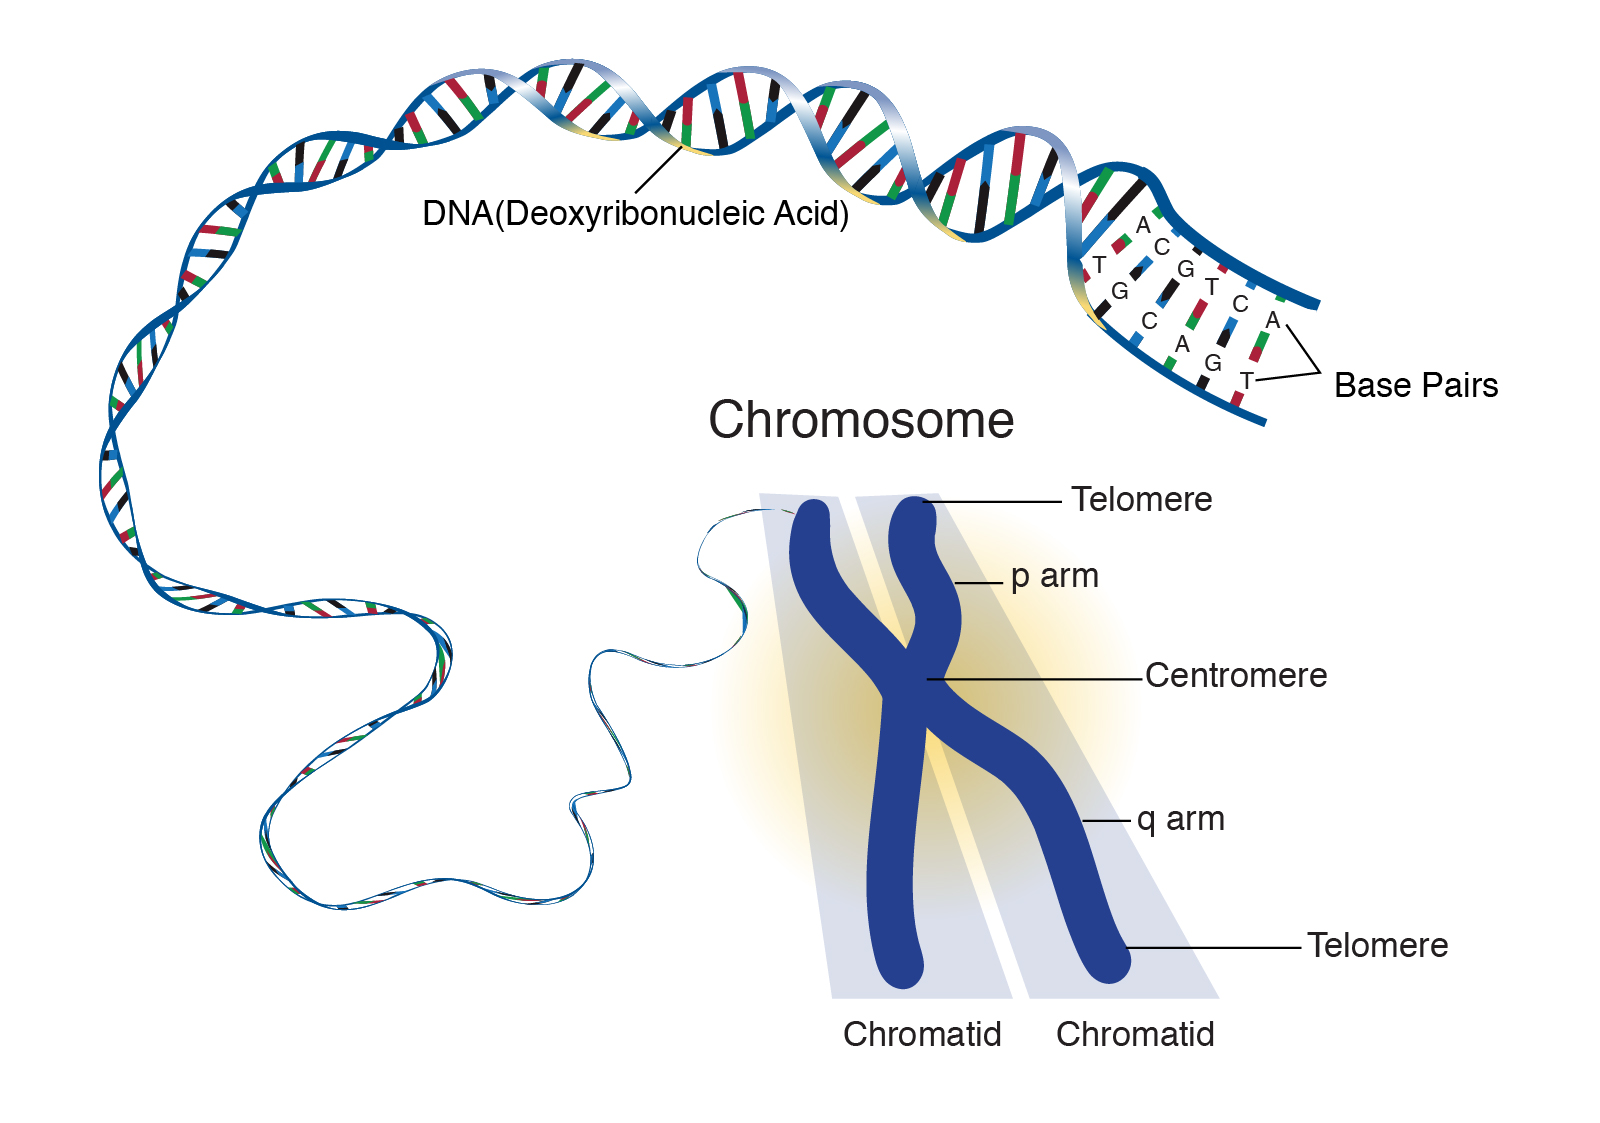
\includegraphics[width=250px]{./img/chromosome.jpg}
		\caption{Umístění nukleotidů v lidském genomu. \cite{chromosome_structure}}
		\label{fig:chrmosome_sekvence}
\end{figure}


\section{Alela a gen}
Alelu můžeme definovat jako variantu genu s nepatrným rozdílemem v sekvenci nukleotidů DNA oproti jiné alele stejného genu. Geny se vyskytují minimálně ve dvou formách (dvou alelách), mnohdy jich, ale může být více. U jednoho člověka můžou být přítomny pouze dvě rozdílné alely daného genu. Gen určuje výskyt nějaké vlastnosti, například tento živočich bude mít oči. Alela pak určuje jakou barvu budou mít.
\\
\\
V případě genu KIR2DL1 mohou být jeho alely 0010101 a 0010102. Zápis genů tak, jak s nimi budeme pracovat může vypadat způsobem zobrazeným v \ref{alela_gen_prikad}. 

\begin{equation}\begin{split} 
   \label{alela_gen_prikad}
   		>KIR:KIR00001\: KIR2DL1*0010101\: 14738\: bp \\
		GTTCGGGAGGTTGGATCTCAGACGTG...
\end{split}\end{equation}

TODO: Když najdu novou sekvenci tak kde je rozdíl jestli je to nový gen nebo nová alela? Neni to tak že na daný pozici v genomu je vždycky gen.. a alela určuje tu vlastnost? A na co je mi teda lotus? 
\\
\\
TODO tohle je asi jen HLA nevím jestli existuje něco jako obecné rozdělení genu a aleli, možná že rozdíl bude jen v tom že těch čísel pak může být za hvězdičkou několik v závislosti o alelu jaké skupiny genů se jedná
Aleli jdou definovány HLA-DRB1* což označuje označuje lokus, následované 4 čísly. 
TODO nevím jestli mám nějak rozebírat to že je tam HLA-DRB1 že tam je tam jednička na konci, já totiž nevím co to znamená
\\
\\
TODO tohle nevím jestli tam dávat: 
Alela zajišťuje konkrétní fenotypový projev genu. U jedince mohou na homologních jaderných chromozomech být přítomny pouze dvě alely. Když jsou v párových lokusech obě alely shodné, jde buď o dominantního homozygota (AA) nebo o recesivního homozygota (aa). Když jsou na párových chromozomech v daném lokusu přítomny různé alely, jde o heterozygota (Aa). Značení alel vzniká dohodou.





\section{Bordel - KIR}
TODO Ligands for NK-cell-activat-
ing receptors are often upregulated by cellular stress
associated with viral infection or tumor development
[26,27] and receptor engagement can lead to the

haplotypycká variabilita
Tzv. „framework“ KIR geny (2DL4, 3DL2 A 3DL3, viz obr. 4)
jsou přítomny prakticky u všech dosud typizovaných jedinců, ale přítomnost ostatních 14 KIR
genů je výrazně variabilní. Tato variabilita v zastoupení je větší pro aktivační KIR geny („S“),
které mají navíc limitovaný alelický polymorfismus. Inhibiční geny jsou obvykle vždy
v genotypu přítomné, ale mají zase extenzívní alelický polymorfismus

Bylo poprsáno celkem 15 exprimovaných KIR genů a 2 KIR pseudogeny


Pokud jde o vazebné partnery KIR (jejich ligandy), pak tyto jsou
známy především pro inhibiční receptory a ve všech případech jde o
HLA specificity I. třídy. Jedná se především o skupinu alel HLA-C alel
lišících se aminokyselinovým 
reziduem na pozicích
 77 a 80 $\alpha$
- helixu molekuly HLA-C (7). Byla publikována rozsáhlá data ukazující
10na význam inhibičních KIR a jejich HLA ligand pro výsledek
transplantace krvetvorných buněk

KIR geny/receptory a jejich vazební partneři (ligandy)
- fryčová ta tabulka tam byla zajímavá, stejná je i v tý disertačce od Jindry odtamtu to asi bude lepší


KIR geny jsou lokalizovány na chromosomu 19q13.4 v oblasti zvané „leukocyte receptor
complex“ (LRC). Pro každý KIR gen navíc existují alelické varianty (Marsh et al, 2002;Hsu
et al, 2002).

Genetická diverzita KIR genů a genotypů připomíná diverzitu HLA
systému. Přestože jsou geny kódující KIR a HLA lokalizované na
různých chromozomech a segregují se tedy nezávisle, existují určité
důkazy alespoň částečné koevoluce obou systémů. Lze tudíž
předpokládat. U HLA restrihované populace lze tedy očekávat
alespoň částečnou redukci v diverzitě KIR genů i genotypů.
U HLA restrihované populace lze tedy očekávat
alespoň částečnou redukci v diverzitě KIR genů i genotypů.

Koevoluce je společný evoluční vývoj dvou či více druhů, při němž dochází k jejich vzájemnému přizpůsobování

Haplotypická variability KIR genů
KIR geny se vyskytují ve dvou hlavních haplotypech A a B, které jsou definovány typem a počtem specifických KIR genů.Ta je způsobena variabilitou v počtu a v typu
zastoupených KIR genů na daném haplotypu
Právě tato
haplotypická diverzita je hlavním důvodem populační diverzity KIR
genů a repertoáru NK buněk.
Neni žádné univerzální kriterium kteréé by je odlišovali

Skipina B je charakterizována přítomností alespoň jednoho nebo víze z následjících genů KIR2DL5, KIR2DS1, KIR2DS2, KIR2DS3, KIR2DS5 a KIR3DS1.

Skupina A je charakterizována absenzí těchto genů. 

Proto mají B více aktivačních KIR než A. A může mít jen KIR2DS4.



\section{bordel}

Je posloupnost písmen představující přimární strukturu reálné nebo hypotetické molekuly čí vlákna DNA, které má kapacitu nést informaci.
označuje se buď nukleotidy nebo nukleové báze
Používaná písmena A, C, G a T reprezentují čtyři nukleotidy ve vláknu DNA – adenin, cytosin, guanin a thymin, lišící se 
typem báze kovalentně vázané k fosfátové páteři. Posloupnost libovolného množství nukleotidů většího než čtyři lze nazývat 
sekvencí. Obvykle se sekvence vypisuje bez mezer, např. AAAGTCTGAC, ve směru 5 -> 3. Vzhledem k biologickým funkcím, které 
mohou záviset na kontextu, sekvence buďto mají anebo nemají smysl a jsou tedy kódující nebo nekódující DNA. Typem nekódující 
sekvence DNA je také tzv. „junk DNA“. TO je z wiki bacha na to.
\subsection{bordel hla}
K typizaci se nejčastěji používá PCR – SSP (PCR se sekvenačně specifickými primery) či
SBT (sequence based typing) technika, v posledních letech se stává zlatým standardem přímá
sekvenace (SBT) HLA genu.
fričová


Aby se určitý gen mohl fenotypově projevit (tj. přepsat se do určitého produktu),
musejí se v jeho lokusu nacházet nejméně dvě alely – jedna pochází od matky, druhá od
otce. HLA-antigeny však mají ve svých genových lokusech abnormálně velké množství
alel, proto tvoří nejpolymorfnější systém v lidském těle.


antigen Jedná se v základu o rozpoznávací molekuly - jsou to vlastně proteiny kódované konkrétním genem, ve výsledku je to to stejné :), protein je vlastně vyjádření genu 

HLA antigeny jsou přítomny na povrchu jsou přítomny na povrchu všech jaderných buněk





 T-lymfocyty rozpoznávají
cizí antigeny v komplexu s vlastními molekulami MHC, což vede k imunitní reakci,
vlastní antigeny v komplexu s vlastními molekulami MHC, což vede k toleranci,
cizí molekuly MHC (transplantační reakce).


Antigeny jsou velmi polymorfní. To znamená, že v lokusu určitého genu na daném
místě DNA, kde se uvedený gen nachází, je možné najít minimálně dvě různé varianty tohoto
genu. Ty se nazývají alely. K tomu, aby měl gen možnost se genotypově projevit, musí jeho
lokus obsahovat dvě alely – jednu od matky a jednu otcovu.
MHC lokusy obecně jsou
geneticky nejvariabilnější kódující lokusy u savců a totéž lze tvrdit i o lidských HLA
lokusech.

HLA antigeny je skupina bílkovin, jsou lokalizovány na povrchu buněk klíčové pro imunitní systém.
Zjednodušeně lze říci že HLA molekuly, imunoglobuliny a receptory T-lymfocytů jsou základem adaptivní imunity člověka

HLA je rozsáhlý komplex genů, které determinují (určují, rozpoznávjí????) povrchové molekuly (antigeny) umístěné v plazmatické membráně buněk

Hlavní fyziologickou funkcí molekul MHC je předkládat antigeny nebo jejich fragmenty buňkám imunitního systému, především T-lymfocytům (prezentace antigenu je prvním předpokladem pro rozvoj imunitní reakce a tím obrany proti napadení mikroorganismy). Pomocí těchto molekul buňky imunitního systému vzájemně kooperují.

\subsection{bordel zbytek}



exprimovaný gen / pseudogeny
takže exprimovaný je ten který se propíše na povrch buňky a pseudogen je ten který se nepropíše na povrch buňky
Pseudogen je sekvence DNA, která je podobná genu, ale nedochází k jejímu přepisování v RNA (transkripci). Pseudogeny vznikají zpravidla určitou mutací, a to zejména v oblasti promotoru, regulační sekvence,[1] nebo sice RNA vzniká, ale je následně degradována.


NK buňky mají schopnost identifikovat molekuly vlastního MHC systému (Major
Histocompatilibity Compex), jmenovitě HLA I. třídy, které jsou normálně exprimovány
prakticky na všech buňkách v těle. Nádorové a některé virem napadené buňky potlačují
expresi HLA I. třídy a tím se brání napadení cytotoxickými T lymfocyty (Restifo, 1993).
Snížená exprese HLA I. třídy činí abnormální buňky citlivé k cytotoxicitě NK buněk (Karre,
1986). Molekuly HLA I. třídy rozpoznávají NK buňky pomocí pozitivních a negativních
13receptorů, které mohou inhibovat nebo naopak aktivovat NK buňky k „zabíjení“

Pokud to můžeme principálně zjednodušit, pak NK buňky neustále
systematicky „zkoumají“ přítomnost či absenci příslušných HLA
ligand pro své KIR receptory. Pokud je příslušný HLA ligand (HLA
molekula) přítomen, pak dojde k vazbě KIR-ligand HLA a jelikož za
normálních okolností vždy inhibiční KIR převládají nad aktivačními,
nedochází ke spuštění cytotoxické reakce NK buněk a takto jsou
„vlastní“ buňky chráněny před cytotoxicitou (viz část A a především D
na obr. 1). Pokud receptory KIR nenaleznou příslušný ligand HLA
(„vlastní“ molekulu HLA), nemůže být cytotoxicita příslušné NK buňky
prostřednictvím inhibičních receptorů KIR a náležitá cytotoxická
kaskáda je spuštěna


Molekuly HLA I. třídy rozpoznávají NK buňky pomocí pozitivních a negativních receptorů, které mohou inhibovat nebo naopak aktivovat NK buňky k „zabíjení“

Tato schopnost destruovat cílové buňky je právě dána vzájemnou
interakcí mezi KIR receptory a příslušnou specifickou HLA molekulou
na povrchu buněk, neboli ligandem KIR receptorů
\\
\\
NK buňky neustále systématicky testují přítomnost čí absenci příslušných HLA ligand pro své KIR receptory. Pokud je přítomen dojde k vazbě KIR-ligand HLA a nedojde k cytotoxické reakci (schopnost níčit buňky) , ochrana vlastních buněk. Pokud je 
nenajdou a je spuštěna cytotoxická kaskáda.
Některé virem napadané buňky nebo nádorové buňky potlačují expresi a tím se brání napadění cytotoxickými T lymfocyty
snížená exprese HLA I. třídy činí abnormální buňky cytlivé k cytotoxicitě NK buněk.

 Molekuly HLA I. třídy rozpoznávají NK buňky pomocí pozitivních a negativních
13receptorů, které mohou inhibovat nebo naopak aktivovat NK buňky k „zabíjení“

NK buňky maji shopnost identifikovat buňky vlastního MHC systému (HLA I.třídy) ktere jsou normálně exprimovány prakticky na všech buňkách v těle. 

Lze-li stručně shrnout, pak NK buňky s potenciálem iniciovat
cytotoxickou aloreakci používají KIRy jako inhibiční směrem k
„vlastním“, zdravým buňkám. Pokud však příslušný vlastní ligand
HLA na cílové buňce chybí, pak je iniciována cytotoxická reakce.
Celý tento koncept interakce KIR/HLA
a mechanismus regulace
cytotoxicity NK buněk se nazývá „missing-self“ hypotéza (3). Tím je
zaručena tolerance NK buněk k „vlastním“ a zdravým buňkám,
naopak alogenní („cizí“) buňky, či buňky s „down“- regulovanou HLA
molekulou (ligandem), což jsou typicky buňky nádorové či buňky
napadené virem, jsou efektivně eliminovány


Stručně lze shrnout, že NK buňky s potenciálem iniciovat cytotoxickou aloreakci používají
KIR receptory jako inhibiční, směrem k „vlastním“, zdravým buňkám. Pokud však příslušný
vlastní ligand HLA na cílové buňce chybí, pak dochází k iniciaci cytotoxické reakce. Proces
interakce KIR/HLA a mechanismus regulace cytotoxicity NK buněk se jako celek nazývá
14„missing-self“ hypotéza (Gasser a Raulet, 2006). Takto je zaručena tolerance NK buněk k
„vlastním“ a zdravým buňkám, naopak „cizí“ alogenní buňky, buňky s „down“ –
regulovaným
HLA ligandem (molekulou), což jsou typicky buňky napadené virem a
nádorové buňky, které jsou efektivně eliminovány

 Tato schopnost destruovat cílové buňky je dána
vzájemnou interakcí mezi KIR receptory a příslušnou specifickou
HLA molekulou na povrchu buněk, neboli ligandem KIR receptorů.


\section{Bordel pro prvni kapitolu}

lymfocyty 
bílá krvinka je leukocyt
- typ bbílé krvinyky 
- T a B lymfocyty - specifická imunita
- NK buňky nespecifická imunita
- vznikají v z lymfatických kmenových buňek v kostní dřeni
Aha takže lymfatické řečiště je více propustné proto to co nejde do cév jde sem pak se to odfiltruje a pak se to vrací do krevního řečiště.

NK je v podstatě lymfocyt a to je typ bílé krvinky.

neutrofilní granulocyty jsou schopny vycestovat z kapilár do místa zánětu
přeměněné monocyty přítomné v játrech v tělních dutinách (hrudní, bříšní), ve slezině vy lymfatických uzlinách a kostní dřeni

KIR
KIR  Je to součástí genu
- řadí se do přirozené (nespecifické) imunity narozdíl od B-buněk a T-buněk.
- NK buňky představují 10-15\% lymfocitů v periferní krvi
- jsou to buňky které reagují rychle a efektivně likvidují především nádorové buňky a buňky infokované virem

NK nemají antigenné specifické receptory, jak rozeznávají abnormální buňky? 
NK buňky identifikují molekuly vlastního MHC systému 

 jmenovitě HLA I. třídy, které jsou normálně exprimovány
prakticky na všech buňkách v těle. Nádorové a některé virem napadené buňky potlačují
expresi HLA I. třídy a tím se brání napadení cytotoxickými T lymfocyty (Restifo, 1993).
Snížená exprese HLA I. třídy činí abnormální buňky citlivé k cytotoxicitě NK buněk (Karre,
1986). Molekuly HLA I. třídy rozpoznávají NK buňky pomocí pozitivních a negativních 
receptorů, které mohou inhibovat nebo naopak aktivovat NK buňky k „zabíjení“

Stručně lze shrnout, že NK buňky s potenciálem iniciovat cytotoxickou aloreakci používají
KIR receptory jako inhibiční, směrem k „vlastním“, zdravým buňkám. Pokud však příslušný
vlastní ligand HLA na cílové buňce chybí, pak dochází k iniciaci cytotoxické reakce. Proces
interakce KIR/HLA a mechanismus regulace cytotoxicity NK buněk se jako 

recptory imunoglobinové (protilátka - protein, který je schopen jako součást imunitního systému identifikovat a zneškodnit cizí objekty - bakterie a viry) v těle. Protilátky jsou nositeli humorální imunity. Jsou to krevní bílkoviny vznikající v mízní tkáni.  povahy nacházejících se na povrchu Natural killers buněk a některých T-buněk (Variabilita v sekvenci).
\\
\\
\textbf{Struktura nukleových kyselin} \\
jen skopírované z %https://www.wikiskripta.eu/w/Struktura_nukleov%C3%BDch_kyselin \\
Nukleové kyseliny (polynukleotidy) jsou tvořeny dlouhými řetězci (mono)nukleotidů, vzájemně spojených fosfodiesterovými vazbami. Řadíme je k tzv.heteropolymérům, neboť jsou sestaveny z různých typů základních jednotek. Tato skutečnost je podstatná pro uchovávání a předávání informace, což je základní funkce nukleových kyselin v organismu. Homopolyméry (např. glykogen) obsahují pouze jeden typ monoméru (v našem případě glukózu), a tak nemohou plnit informační funkci.




\chapter{Sekvenační metody získávání DNA dat}
Sekvenování DNA, někdy pouze sekvenování, jsou biochemické metody, kterými se zjišťuje pořadí nukleotidů (A, C, G, T) v sekvenci DNA. Sekvenační metody se liší zejména délkou řetězce, kterou dokáží zpracovat, cenou a rychlostí sekvenace. Pro porovnání sekvenování celého genomu sangorovo metodou by stálo několik milion dolarů a trvalo zrhuba 10 let. Při použítí dnešních metod by cena byla zhruba tisíc dolarů. Největším problémem u sekvenování je, že sekvence vzniklé ze sekvenátoru jsou jen kousky které je třeba poskládat zpět. Většina sekvenačních metod využívá vlasnosti přitahováním báze do páru pouze jednou konkrétní bází. To znamená že se adenin vždy páruje s thyminem a cytosin se vždy páruje s guaninem. Z těchto párů vzniká již známá dvojitá šroubovice DNA. Při sekvenování je možná se často setkat, že se sekvenuje jen kónkrétní kus DNA, který je zrovna potřeba. \cite{sekvenovani_ziva}
\\
\\
TODO možná tady ještě napsat něco o přípravě na sekvenování - je to dyžtak v tý přednášce co nám řikala na FAV
\section{Sanger sequencing}
Sanger sekvenování využívá možnosti namnožení řetězce díky vzájemnému přitahování konkrétních bází. V prvním kroce replikace jsou nastříhané řetězce rozděleny na dvě vlákna. Lze si představit, že tyto dvě oddělená vlákna jsou dána do směsy, kde plavou jednotlivé nukleotydy spolu s upravenými nukletidy, které nesou specifickou fluorescenční barvu a za které neni možné nic navázat. Následně za pomoci střídaní teploty volně plující nukleotidy tvoří postupné páry s řetězcem, který chceme namnožit. Pokud se povede celý řetězec namnožit je odtržen a může se dále množit. Postupně ale bude docházet k navazováním nukleotidů s fluorescenční barvou. Tím se vytvoří nekolik různě dlouhých sekvencí zakončených označeným nukleotidem. Podle jeho barvy je možné poznat o jaký nukleotid se jedná. Následně jsou za pomoci elektorforézy seřazeny v gelu podle délky. Elektroforéza rozděluje různě dlouhé sekvence na základně odlišnosti pohybu v elektrickém poly. Kratší doputují dále než delší. Pomocí sanger metody je možné sekvenovat řetěce dlouhé až 1000 bází.   

\begin{figure}[H]		
		\centering
		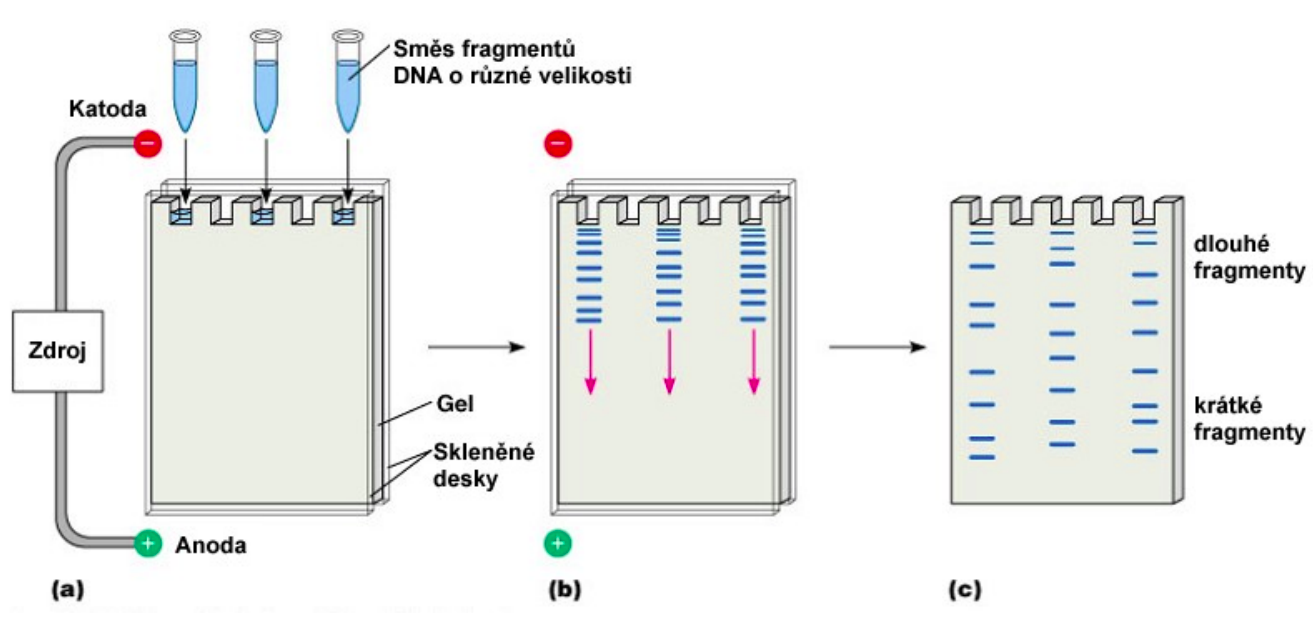
\includegraphics[width=\textwidth]{./img/elektroforeza.png}
		\caption{Elektroforéza. \cite{elektroforeza_img}}
		\label{fig:elektroforeza}
\end{figure}

 
TODO možná sem ještě přidat obrázek tý destičky.. ale zatím se nenašla nějakej hezkej.
 
 
\section{NGS next-generation sekvenování}
Next-generation sekvenování někdy označováno jako metody druhé generace jsou v porovnání se Sangerovo sekvenováním rychlejší a levnější, na druhou stranu ale dokáží zpracovávat jen řetězce dlouhé 100 až 500 bází, mají menší přesnost a časteji chybují. Jejich rychlost spočívá především ve schopnosti detekovat přidávání bází jednu po druhé a zároveň sekvenovat tisíce až miliony rozdílných molekul DNA najednou. 
\\
\\
Všechny tyto metody si předpřipraví řetězce nastříháním na krátké části a připevenín takzvaného adeptéru na jejich konec. Adaptér je krátká molekula DNA, která slouží k uchycení sekvenovaného úseku na pevný povrch. Řetězce DNA jsou namnoženy díky čemuž vzniknout klastry identických molekul koncentrovaných v jednom místě. Díky tomu je posílen signál, který by z pouhé jedné molekuly nebly dostatečně silný. Tento signál je zachycen kamerou. Jeden z důvodů popularity NGS metod jsou i cenově dostupné stolní sekvenátory.
 

\subsection{454 sekvenování a Ion Torrent}
454 sekvenování bylo vypuštěno do světa v roce 2005. Dokáže analyzovat více než milion molekul DNA najednou a délka každé jednotlivé sekvence se pohybuje okolo 700 až 1000 bází.
\\
\\
V prvním kroku sekvenování je molekula DNA přichycena na malou "kuličku" na jejimž povrchu se postupně namnoží až kuličku zcela pokryjí identické molekuly DNA. Následuje vložení kuličky i s DNA do jedné z milionů komůrek na destičce s reakční směsí. V určitém momentě je do této směsy přidán vždy jen jeden typ báze. Mezi jednotlivými fázemi přidávání určité báze jsou přebytečné nukleotidy z předešlého kroku odstraněny. To znamená že v reakční směsy je vždy jen jeden typ nukleotidů. Během vložení každé nové báze do rostoucího řetězce DNA je uvolněna molekula zvaná pyrofosfát.  Tento pyrofosfát se následně spustí několik chemických reakci. V poslední fází enzym luciferáza vydá světelný záblesk, který je možné zachytit citlivou kamerou.  Tento postup se nazývá pyrosekvenování. V případě, kdy je do řetězce přidáno několik stejných bází za sebou, například gen obsahuje podřetězec AAA, je vyzářeno, v našem případě, třikrát více světla než v případě jedné přiřazené báze. Kamera snímá celou destičku a na základě. která komůrka se rozsvítí pozná kde přoběhlo přidání báze. Intenzita světla pak určuje kolik bází bylo přidáno na jednou. 
\\
\\
Sekvenování Ion Torrent funguje na podobné princupu sekvenování s rozdílem, že místo světla se měří změna pH v reakční směsy. Podle intenzity změny pH lze pak poznat kolik nukleotidů bylo přidáno do rostoucího řetězce.
\\
\\
Hlavní slabinou těchto dvou metod je značná chybovost při přidání mnoha stejných nukleotidů do řetězce za sebou. Například pří přidání 10 A, nebude odpověď jednoznačná zda je to 10 A nebo 9.


\subsection{Illumina}
Při sekvenování pomocí Illumina jsou páry dvoušrobovice rozděleny na dva řetězce. Jednotlivé řetezce jsou následně přichyceny na malou destičku pomocí adaptéru. Každý řetězec se následně opakovaně množí až na destičce vznikne několik shluků. Přidání jedné molekuly ke druhé probíhá obdobně jako u Sanger sekvenování. Každý shluk tvoří jednu skupinu vzájemně identických řetězců. Mezi volné nukleotidy jsou opět zahrnuty nukleotidy označeny fluorescenční barvou za které nelze nic navázat. Oproti sangerovu sekvenování je ale tato blokace vratná a po přečtení citlivou kamerou dojde k odstranění blokující části molekuly. Počítač si pak následně zpětně spočítá co to bylo za barvu (nukleotid.) 


\subsection{SOLiD}
SOLiD (Sequencing by Oligonucleotide Ligation and Detection) se spoléhá na enzym ligáza, který umožňuje připojení jednořetězcových molekul k stávajícím řetězcům. K teplátu jsou přidávány takzvané sondy, což jsou kousky DNA. Sondy začínají všemi možnými dvojkombinacemi čtyř základních nukleotidů. V součtu je 16 sond. Na každé sondě je jedna ze čtyř flurescenčních barev. V jednotlivých krocích jsou sondy připojeny k rostoucímu řetězci. Následně je přečtena fluorescenční barva, která je odstraněna a může se tak navázat další sonda. Z výsledného signálu lze pak ododit výslednou sekvenci DNA.


TODO Je tam hezká tabulka porovnání tak by se sem mohla taky dát
\section{Metody třetí generace}
Velkým rozdílem oproti druhé generaci je že DNA templát není před sekvenování namnožen a je čten pouze z jedné původní molekuly. Existuje například PacBio od Pacific Bioscience, který k detekci využívá fluorescenčně značené nukleotidy. Díky jeho vysoké citlovosti je možné v reálnám čase zachytit přidání i jediného nukleotidu do jediného řetězce DNA. Další zástupce je Oxford Nanapore jehož výhodou je jeho velikost. Oxford využívá odlišného tvaru bází. Obě metody jsou schopné přečíst přes 10 tisíc bází v rámci jedné analyzované molekuly DNA. 






\section{Read}
Read je sekvence bází odpovídající celému genomu či nějaké jeho části. Ready jsou typický výstup sekvenačních technik, kdy výstupem je sekvence nukleotidů o kterých nikdo neví co znamenají. Může to být gen, část genu nebo několik různých genů. Význam readu (o jaký gen se jedná) se zjišťuje zarovnáváním, kdy se daná sekvence porovnává vůči referenčnímu genu.
-wiki  


\section{Bordel}
SANGER
Vybraná sekvence se vloží do reakční směsi s radioaktivně označným primer  

Během procesu replikace jsou řetězce rozděleniny na dvě vlákna. 
V praxi to není tak snadné a hrají roly i další proteiny. 
Mezi nukleotydi plavou i uprvené nukleotidy které nesou specifickou fluorescenční barvu a za ně už neni možné aby s něco nevázalo.  Podle barvy poznáme o jakou bázi se jedná. 
Náhodný přerušováním syntézy vznikají různě dlouhé molekuly. 

výhody dlouhá délka sekvencí které se dají sekvenovat jedinou reakci a vysoká přenost čtení
v rámci celého procesu dochází k sekvenování pouze jednoho úseku DNA 
vysoká cena a nízká rychlost
 K sekvenaci se použtívá gelová elektrofézy
 použitelná k sekvenování krátké sekvence jednovláknové DNA. 
 využívá biologického procesu replikace DNA
 Vybraná sekvence se vloží do reakční směsi s radioaktivně označným primer
 rozdělí se to na přibližně 
 namnoží se to .. 
 pak se to hodí do něčeho co nakonci svítí tak ty se navážou na příslušnej konec.. 
 pak to pustíme do gelu .. 
 nejkratší projedou nejdál
 nejdelší zůstanou co nejblíž a podle toho pak sestavuju jak ta sekvence vypadá
Sekvenování DNA je souhrný termín pro biochemické metody, jímiž se zjišťuje pořadí nukleových bází (A, C, G, T) v sekvencí DNA. Tyto sekvence jsou součástí dědičné informace v jádru.
Adenin s thyminem a cytosins s guaninem.

zjišťvání přímární struktury nukleových kyselin (sekvencování)
Někdy se sekvenují pouze jisté části genomu které mají pro výzkumníka v daném okamžiku význam.
Užitečné nejen ve výzkumu ale i v diagnostice nemocí či forenzní medicíně. 


454 
, kde probíhá sekvenační reakce na principu pyrosekvenování.  

 Pyrosekvenování se za -
kládá na skutečnosti, že během vložení
každé nové báze do rostoucího řetězce
DNA se uvolní molekula zvaná pyrofosfát
(proto pyrosekvenování). Uvolněný pyrofosfát se posléze stane součástí několika
na sebe navazujících enzymatických reakcí, na jejichž konci čeká enzym luciferáza
Ten vydá světelný záblesk, jenž lze za -
chytit vysoce citlivou kamerou


 Při 454 sek -
venování je v určitém momentě přidán do
reakční směsi vždy pouze jeden typ báze
a v okamžiku, kdy je tato báze vložena do
rostoucího řetězce DNA, dojde přes uvolněný pyrofosfát a luciferázu ke světelnému
záblesku. Pokud je do rostoucího řetězce
DNA zařazeno několik stejných bází za se -
bou, např. když DNA molekula templátu
obsahuje sekvenci AAA a je tedy přidáno
třikrát T, vyzáří se třikrát více světla než
v případě přiřazení jednoho T

. Kamera
snímá celou destičku a podle toho, která
komůrka se rozsvítí, pozná, kde proběhlo
přidání báze, a podle intenzity světla ko -
lik bází bylo přidáno najednou

Nukleotidy jsou přidávýny jeden po druhém a mezi jednotlivými dochází k odtranění přebytečných nukleotidů.
takže v rekční směsy je vždy jen jeden typ nukleotidů.


Ion Torrent je na podobném principu jako pyrosekvenování
ale neměří světlo ale změnu pH v reakční směsy. Pod
podle intenzity změny pH

protože spolehají na sílu signálu aby věděli kolik bází bylo přidáno  nejednou mají obě metody problém se čtením dělších řetězců obsahující práce jen jednu bázi například AAAAA. nebude jednoznačná odpověď zda je to 9 A nebo 10.

Ilumina
Dokáže sekvenovat až 900 miliard? bází najednou. 
potřebuje kratší sekvence - stovky bází
pomocí adaptéru přichyceny molekuly DNA na malou destičku

Každá molekula DNA se pak opakovaně namnoží, až na destičce vznikne
mozaika milionů klastrů, přičemž každou
skupinu tvoří vzájemně identické molekuly. Vlastní sekvenační proces pak využí -
vá podobného mechanismu jako Sange -
rovo sekvenování, kdy jsou do rostoucího
řetězce zařazeny báze s navázanou fluorescenční barvou (každé písmeno má speci -
fickou barvu), které syntézu zastaví.

tato blokace je orpoti sangerovi vratná
 popřečtení citlivou kamerou dojde k odstranění fluorescenčního značení i blokující části molekuly
 a může se pokračovat
 
 kamera snímá celou destičku
 a podle rozdílné fluorescence pozná co bylo přidáno u každého z milionů skupin
 
 počítač si to pak zpětně přechroupa krok po kroku.
 

nejčatější chybou je špatně přečtené písmenko. 
jinak má 99 procentní úspěšnost

\subsubsection{Read bordel}
In DNA sequencing, a read is an inferred sequence of base pairs (or base pair probabilities) corresponding to all or part of a single DNA fragment. A typical sequencing experiment involves fragmentation of the genome into millions of molecules, which are size-selected and ligated to adapters. The set of fragments is referred to as a sequencing library, which is sequenced to produce a set of reads. Je to z wiki zase
\\
\\
V DNA sekvenování, read je odvozená sekvece párů bází odpovídající celému fragmentu DNA nebo jeho části
To znamená že read je kus DNA který by mohl odpovídat nějakého konkrétnímu genu? 
\\
\\
Pak tam ještě bylo psaný něco o read lenght
Sekvenační technologie se liší? v délce vyrobenybch readů. 
Ready díkjy 20-40 párů bází (bp) jsou ultrakrátké
Typická sekvenační metoda vytváří ready délky 100 až 500 bp

DNA knihovny - podle wikiskripta
DNA knihovny jsou kolekce klonovaných DNA fragmentů genomu určitého organismu (cDNA), které jsou skladovány uvnitř hostitelských organismů (zejména bakterií). cDNA (copy DNA, complementary DNA) je získávána přepisem z mRNA pomocí enzymu reverzní transkriptázy.

Kvalita knihovny
Při přípravě sekvenční knihovny je důležité získat co nejvyšší úroveň složitosti. Jinými slovy, je důležité, aby konečná knihovna co nejvíce odrážela jedinečnost výchozího materiálu. Tento výsledek lze získat především omezením počtu segmentových duplikací. Čím kratší jsou fragmenty, tím vyšší je pravděpodobnost, že jsou fragmenty méně specifické a mohou se zarovnat na více než jednom lokusu referenční sekvence. Složitost knihovny lze tedy v podstatě měřit procentem duplicitních čtení, které jsou přítomny v sekvenčních datech

Sekvenování mRNA s použitıím NGS technologií umožňuje měření genové exprese celého
transkriptomu. Postup a provedení RNA-seq experimentu je znázorněn na obr. 14.
Prvním úkolem je vyčistit zkoumaný vzorek o rRNA, tRNA a mitochondriální RNA,
které u prokaryot i eukaryot tvoří přibližně 75 procent všech RNA molekul. Navzdory použití
purifikačních metod, mezi které patří například poly(A)purifikace a DNS normalizace,
sekvenační data mohou obsahovat menší množství těchto RNA molekul [59]. Ty mo-
hou být odfiltrovány v následujícíh krocích bioinformatickými postupy. Zbylá mRNA
je poté nastříhána na menší části, a je z ní připravena knihovna krátkých fragmentů s
navázanými adaptory. Ty jsou poté sekvenovány sekvenačním přístrojem a jako výsledek
získáme tzv. ready. Anglické slovo ’read’ značí datovou reprezentaci krátké sekvence
DNA obvykle 50-150 bp dlouhou, která byla vyprodukována sekvenačním přístrojem.
Samotné ready však nemají žádnou vypovídající hodnotu, a proto jsou dále bioinformat-
icky zpracovány. Namapováním na referenční sekvenci zjistíme jejich genomickou pozici,
ze které byly odvozeny. Většina readů je namapována na exony, což jsou transkripčně
aktivní jednotky, a pouze malé množství readů je namapováno na transposony. Ready
které nejde namapovat v celku, jsou rozděleny na menší části a ty jsou namapovávány
zvlášť. Rozdělené ready umožňují jednodušší identifikaci mezer mezi exony (angl. splice
junctions)
tohle je z tý diplomky single-pair

\chapter{Analyza dostupných bioinformatických nástrojů pro zpracování NGS dat}
\section{Referenční geny}
Referenční geny byly převzaty z IPD-KIR \cite{imgt_hla_database} konkrétně soubory ve formátu $fasta$ uloženy ve stejnojmené složce. Jednotlivé soubory jsou pojmenovány genem který obsahují např. $KIR2DL1\_gen.fasta$. Každý soubor představuje všechny dostupné alely konkrétníhé genu.
\\
\\
Kromě souborů $*\_gen.fasta$ obsahuje složka $fasta$ také soubory $*\_prot.fast$ a $*\_nuc.fasta$. Soubor $*\_prot.fast$ obrahuje sekvenci proteinů, nuc obsahuje nucleotidy a gen obsahu genomic DNA sekvence
\\
\\
TODO já vlastně nechápu jakej je rozdíl mezi nuc a gen? 
\\
\\
All files in this folder are provided in the FASTA sequence format. Please note the FASTA format contains no alignment information.

Files designated “X\_prot.fasta”, where X is a locus or gene, contain protein sequences. Please note that alleles that contain non-coding variations may be identical at the protein level. 

Files designated “X\_nuc.fasta”, where X is a locus or gene, contain the nucleotide coding sequences (CDS). Please note that alleles that contain non-coding variations may be identical at the CDS level.

Files designated “X\_gen.fasta”, where X is a locus or gene, contain genomic DNA sequences. Please note for alleles that do not possess genomic sequences, there will be no entry in the file.

\subsection{Vytvoření testovacího haplotypu}

TODO navíc hned když se podívám na 3DL3: 00402 tak tam mám dvě možnosti
TODO a co když tam nějakej není, tak prostě pokračuju tím dalším, nebo se tam něco dává jako mezera? Myslím když jste třeba napsala 2DL5B:
TODO Co je 2DP1, ve FASTA jsem je nenašla tak jsem to skopčila z \url{https://www.ebi.ac.uk/cgi-bin/ipd/kir/get_allele.cgi?2DP1*0020103} - p značí pseudogen
A prej by měli být v KIR-gen.fasta ale já to tam za boha nemůžu najít
jo tak tam je v tom KIR\_gen fasta
ale nahoře jsou i jiný co asi úplně nejsou pesudogeny tak to moc nechápu ..
 
to děláte správně, jen musíte vytvořit KIR haplotyp, který podšoupnete tomu ARTu, nejenom jeden konkrétní KIR, aby Vám vytvořil ready, tj. např. kombinaci (tophle je jedna známá linie, sloučíte si ty KIRy za sebe):
3DL3: 00402, 00802
2DS2: 00101
2DL2: 00301
2DL3: 001
2DL5B:
2DS3:
2DP1: 00201
2DL1: 00302
3DP1: 007, 00901
2DL4: 00102, 00501
3DL1: 01502
3DS1: 01301
2DL5A: 001
2DS3:
2DS5: 00201
2DS1: 00201
2DS4: 001
3DL2: 0020105, 0070102

\section{Biopython}
normálně přes pip3 install biopython

tak to vypadá že i ten biopython umí aligned a že to dělá přes to Burrows wheeler aligner 
\section{ART}
ART (next-generation sequencing read simulator) je sada simulačních nástrojů, které generují syntetické ready, jako kdyby byli získány sekvenováním pomocí NGS. Nástroj ART dokáže simulovat ready ze sekvenátorů Illuminas, 454 společnosti Roch a SOLid od společnosti Applied biosystém. Ready, vytvořené nástrojem ART jsou používány pro testování a analýzů nástrojů zpracovávající právě NGS sekvence jako například zarovávání (nástroj Bowtie). 
\\
\\
ART je implementován v jazyce C++ a je dostupný s licencí GPL verze~3 pro operační systémy Linux, MacOs a Windows. Je možné ho použít i jako C++ package. Pro jeho spuštění je nutní mít nainstalovaný compilator GNU g++ 4.0 nebo vyšší a knihovnu GNU gsl. 
\\
\\
Data získána z FN Plzeň byla sekvenována nástrojem Illuminas proto i syntetické ready budou simulovat tento sekvenátor.    
 Výstupy se čtou ve formátu FASTQ a zarovnání ve formátu ALN. může generovat zarovánávání také ve formátu SAM nebo UCS BED. \cite{art}




\subsection{pokus to nejak spustit}
Takze kdyz otebru hlavni readme tak mi to riká že tam jsou read me pro jednotlivy verze sekvenatoru ..

pak se to musí skompilovat 

./configure --prefix=\$HOME
	       	make
	       	make install	 
	 
teď mě zajímá ta ilumia tak podle readme ilumina tak můžu vlést do složky examples a tam pustit skript run\_test\_examples\_illumina.sh , tak tam jsou 4 příklady použití 
a pokud asi všechno dobře porběhne tak se mi zobrazí pár nových souborů ve složce examples.. 

FASTQ - *.fq data file s ready. pro paired-red simulator
*1.fq obsahuje data pro rvní ready a *2.fq rdu druhy ready

tohle nějak funguje
MSv3 tam musím dát abych to mohla dostat na délku readu 250 a p znaci ze to je paired.. 
tak se má používát MSv1
$art_illumina -ss MSv3 -sam -i amplicon_reference.fa -p -l 250 -f 10 -m 300 -s 10 -o moje_art_data$
Tohle používej:
$art_illumina -ss MSv1 -sam -i amplicon_reference.fa -p -l 250 -f 100 -m 300 -s 10 -o moje_art_data$

\subsection{FASTQ}
Sekvenační přístroje produkují data ve formátu FASTQ takže i ART musí logicky generovat tenhle formát.
Pokud jsou ready v páru tak je na konci .1
a druhý read z páru tam má .2 to jsem u těch svých přímo nenašla 

ale máš teda tři druhy single end, paired-end a matepair. 

FASTQ obsahuje obě základy sekvence ?? both sequence bases a kvality skore je to v následujícím formátu
@read\_id
sequence read
+
base quality scores je kódovany by ascii code of a single character, kde je kvalita rovná score to ascii code character minus 33. chápu proč tam je to -33 protže když se podíváš do asci tabulky tak je tam od 33 první normální znak jinakjsou tam divný .. 
takže třeba otazník je v asci na 63 takže -33 takže má ohodnocení kvality 30
jen by mě teda zajímalo v jakým sme intervalu? - je 45 v asci a nevím jestli to je teda od 0 do 100?  a teda nejvyšší číslo znamená nejkvalitnější a nejmenši míň kvalitní? Podle tý diplomky to tak je že čím vyšší číslo tím kvalitnější a většinou je to od 0 do 40 jen zřídka to překročí hodnotu 60, když je tam 10 tak to znamneá že jedna báze z deset je špatně.. když je tam 30 tak to znamená že jedna z 1000 je špatně.
já tam mám třeba F a to je 70.

example:
		@refid-4028550-1 
		caacgccactcagcaatgatcggtttattcacgat...
		+ 
%		????????????7?????<??>??=&?<<?-<?0?...

ALN - zarovnání readů
zase *1.aln pro první a *2.aln pro druhý
soubor je rozdělen na hlavičku a body část
obsahuje hlavičku a v tý hlavičce je jakým příkazem byl soubor vygenerován a reference na sequnce id a jejich délku
@CM tag pro příkaz a
@SQ pro reference sequence
Hlavička vždycky začíná s 
%##ART a končí s ##header end

		HEADER EXAMPLE

%		##ART_Illumina  read_length     35
%		@CM     ../art_illumina -i ./testSeq.fa -o ./single_end_com -l 35 -f 10 -sam -rs 177
%		@SQ     seq1    7207
%	       	@SQ     seq2    3056
%		##Header End
		
v body jsou všechny zarovnání 
%		>ref_seq_id	read_id	aln_start_pos	ref_seq_strand
%	       	ref_seq_aligned
%	       	read_seq_aligned 
	    
	    aln\_start\_pos označuje počáteční pozicí v referenci sekvence, je vždy relativní vzhledem k vláknu referenční sekvence
	    To znamená že aln\_start\_pos plus (10) vlákno je odlišný od  aln\_start\_pos minus (-) vlákna.. ???? WHAT???
	    
		ref\_seq\_aligned je zarovnaná oblast referenční sekvence, která může být plus vlákno nebo mínos vlákno referenční sekvence
		ref\_seq\_aligned je zarovanný read, který je vždy ve stejné orientaci jako stejný read v odpovívajícím fastq suboru.  
		
		
			    
	    
	       	
		aln\_start\_pos is the alignment start position of reference sequence. aln\_start\_pos is always relative to the strand of reference sequence. That is, aln\_start\_pos 10 in the plus (+) strand is different from aln\_start\_pos 10 in the minus (‐) stand.  
	
		ref\_seq\_aligned is the aligned region of reference sequence, which can be from plus strand or minus strand of the reference sequence. 
		read\_seq\_aligned is the aligned sequence read, which always in the same orientation of the same read in the corresponding fastq file. 

SAM je standardní formát pro NG sekvence ready zarování
BED o tom tam nic neni jen 
NOTE: both ALN and BED format files use 0-based coordinate system while SAM format uses 1-based coordinate system.

pak jsou tady 4 doporučené použití
$art_illumina [options] -ss <sequencing_system> -sam -i <seq_ref_file> -l <read_length> -f <fold_coverage> -o <outfile_prefix>$
$art_illumina [options] -ss <sequencing_system> -sam -i <seq_ref_file> -l <read_length> -c <num_reads_per_sequence> -o <outfile_prefix>$
$art_illumina [options] -ss <sequencing_system> -sam -i <seq_ref_file> -l <read_length> -f <fold_coverage> -m <mean_fragsize> -s <std_fragsize> -o <outfile_prefix>$
$art_illumina [options] -ss <sequencing_system> -sam -i <seq_ref_file> -l <read_length> -c <num_reads_per_sequence> -m <mean_fragsize> -s <std_fragsize> -o <outfile_prefix>$

pak tam máš parametry 

a jak dlouhý chceme simulovat ready? 



\subsection{bordel}
ART is freely available to public. The binary packages of ART are available for three major operating systems: Linux, Macintosh, and Windows. ART is also available as Platform-independent C++ source packages. Each package includes programs, documents and usage examples.

ART simuluje ready napodobobáním skutečných procesů sekvenování s empirickým chybovým modelem nebo quality profiles summarized from large recalibrated sequencing data
ART může také simlovat čtené pomocí uživatelského vlastního read arror modelu nebo quality profiles

TODO - tohle úplně nechápu ART podporuje simulaci jedno párových, dvou párovcýh tří hlavních komerčních sekvenčních platfoem 
Výstupy se čtou ve formátu FASQ a zarování ve formátu ALN. 
ART může také generovat zarovnávání ve formátu SAM nebo UCSC BED
ART lze použít společně se simulátory varient genomů VarSim 
\\
to je odtud %https://www.niehs.nih.gov/research/resources/software/biostatistics/art/index.cfm
454 sekvenování je pyrosekvenování, které cycklicky testuje přítomnost každého ze čtyř nukleotidů DNA (T, A, C, G)

SOLid ke kódování 16 různých dinukleotidů používá čtyči fluoresenční barevná barviva, každé barvivo kóduje čtyři dinukleotidy
 


tak jsem stáhla normálně nejnovější verzi z niehs.nih.gov a podle instrukcí co byli v souboru INSTAL dala % ./configure && make && make install


musí se brát v potaz že z toho generátoru nikdy nebudou data taková jako reálná.. realná budou horší 




\section{Bowtie}
Bowtie je rychlý a paměťové efektivní nástroj pro zarovnávání krátkých sekvencí DNA na velké genomy. Indexace pomocí Burrows-Wheelere transformace dovoluje zarovnávání více než 25 milionů readů za CPU hodinu pro lidský genom s pamětí příblížně 1.3 gigabajtů. Bowtie přidáváa k Burrows-Wheeler technice backtracking algoritmus pro sledování nekonzistence. ??


\subsection{Bordel}
Bowtie je napsanej v c++ a používá knihovnu seqAn

Na lidském genomu je nástoj Bowtie v porovnání s nástoji Maq a SOAP rychlejší. 
Citlovost má bowtie srovnatelné s nástojem SOAP a o něco menší než Maq. Ale je možnost pomocí příkazové řádky zvýšit citlivost na úkor rychlosti běhu progamu.
Oproti SOAP bowtie potřebuje méně paměti 1.3 GB RAM. 
Bowtie zarovnává  25 milionů readů za hodinu. může běžet paralelně.

indexi vytváří permanentní a lze je použít napříč běhy 
pro lidský genom je to 2.2 GB takže ho lze distribuovat přes internet
rychlost a malá paměť způsobuje především Burrows wheeler v kombinaci s backtrackingem.

Podrporuje standardní vstupní formáty FASQ a FASTA.

Bowtie je open source.

 
na stránkách elixir-europe což je oragnizace co má dávat dohromady všechny vědecký veci a bla bla.



Tak tam je přímo Bowtie \cite{bowtie}

\subsection{Bowtie 2}
Note that SOAP2 and Bowtie do not permit gapped alignment of unpaired reads.
 memory footprint of Bowtie 2 (3.24 gigabytes)
 Bowtie 2 by mělo být vhodnější pro delší ready než Bowtie1.
 We extracted a random subset of 1 million reads from each and aligned them with BWA-SW and Bowtie 2. We did not align with Bowtie, BWA or SOAP2 because those tools are designed for shorter reads.
Bowtie už je překonanej nejenom Bowtie2 ale i BWA.
Bowtie2 je podle studie znatelně lepší než Bowtie, SOAP2.
tyhle výsledky jsou na syntetických readech

vypadá to že bowtie 2 už nepoužívá tamten index ale používá nějaký Full-text minute index–assisted search což vypadá že je kombinace burrows wheelera a ještě něčeho.
We found that Bowtie 2, a method that combines the advantages of the full-text minute index and SIMD dynamic programming, achieved very fast and memory-efficient gapped alignment of sequencing reads

je zase open source
\cite{bowtie2}


šla jsem přes docker docker image ls - zobrazi vsechny image pak docker run a ID image
sudo docker run -i -t 3c2b9a287f82 /bin/bash
sudo docker ps -a

Tak jsem nakonec žádnej docker nepotřebovala a stáhla jsem to tady %http://bowtie-bio.sourceforge.net/tutorial.shtml
 po kliknuti na bowtie binary release.

na strance 25.4 je řečeno o hledání tch nejlepších zarovnání a je tam možnost --best ale že je dvakrát nebo třikrát pomalejší než normální mod.. a jde o to že najde první přijatelný a to označní kdežto při tom best prohledá co nejvíc a hledá to nejlepší i mezi těma přijatelnýma a to je pomalý.

takže zarovnání by mohlo být teoreticky namapování na referenční gen???

\subsection{bordel}
tak jsem  to stáhla dala do složky a musela jsem teda nastavit proměnou prostředí 
export BT2\_HOME=$/home/kate/Dokumenty/FAV/Diplomka/existujicisw/bowtie2-2.4.1-linux-x86_64/$
pak jsem pustila tohle: 
\$BT2\_HOME/bowtie2-build \$ $BT2_HOME/example/reference/lambda_virus.fa lambda_virus$
a nakonec se mi vytvořili nějaký nový soubory lambda virus 1 atd.. v tom bowtie 2 adresáři

dělala jsemt o podle tohohle webovky %http://bowtie-bio.sourceforge.net/bowtie2/manual.shtml#getting-started-with-bowtie-2-lambda-phage-example


z bowtie pak teda leze asi SAM formát
\subsection{Popis problému}
\subsubsection{SAM}
1. název readu který je zarovnáván

2. Sum of all applicable flags. Flags relevant to Bowtie are:
součet všechn aplikovaných (příslušných flags). Flagy relevantní k bowtie jsou: 
1 - read je jeden z páru
2 - zarovnání je one z paired proper (The alignment is one end of a proper paired-end alignment)
4 - read má reported alignments
8 - read je jeden z páru a má reportovaný zarovnání
16 - zarování je obrácená reference vlákna
32 - The other mate in the paired-end alignment is aligned to the reverse reference strand
64 - read je mate 1 in a pair
128 - read je mate 2 in a pair

Thus, an unpaired read that aligns to the reverse reference strand will have flag 16. A paired-end read that aligns and is the first mate in the pair will have flag 83 (= 64 + 16 + 2 + 1).

3. jméno referecnce ze které zarování patří
4. 1-based offset into the forward reference strand where leftmost character of the alignment occurs 1-based odszaneí v následující referenci 
5. kvalita mapování
6. CIGAR reprezentace zarovnání
7. název reference kde je zarovnán kamarád 
8. 1-based zarování ofsetu k nálsedující refenrenci 
9. Odvozená délka fragmentu. Velikost v závoru je že se mate nachází předtím. 0 že jsem nezarovnali mate
10. read sekvence
11. ASCII encoded read kvalita, stejné jako u FASTQ
12. optional pole


SAM Sequence Alignment Map format), respektive jeho binárně
komprimovaná verze BAM (z angl. Binary Alignment Map format).
\section{IGV}
nakonec jsem to pustila přes IGV ale stejně se tam museli ty indexi dodělat
%java --module-path=lib -Xmx4g @igv.args --module=org.igv/org.broad.igv.ui.Main
a musim byt ve slozce 
$~/Dokumenty/FAV/Diplomka/existujicisw/IGV/IGV_Linux_2.8.0$

když to otevřeš tak možná občas vypadá že tam nic neni tak musíš vybrat konkrétní úsek nahoře z toho rolovátka
Možná by se pak dalo udělat to že ty víš že tam může být maximálně dva z toho jednoho KIR souboru.. jako že může mít maximálně dvě alely z jednoho souboru
No akorát co mi to udělá když bude mít dvě stejný? 

\chapter{Seznam zkratek}
HLA
KIR
NK
sekvence DNA cytosin, adenonin atd
DNA (Deoxyribonuklenovou kyselinu)
co ty formáty souboru?

\chapter{Výkladový slovník pojmů?}
WHO
český národní registr 
možná zmínit národní registr
genotyp 
fenotyp tyhle kraviny
Genotyp pro danou chromozomální oblast se pak u většiny lidí skládá ze dvou haplotypů).
genom kompletní sekvence daného organismu
% 
% PRO ANGLICKOU SAZBU JE NUTNÉ ZMĚNIT
% CITAČNÍ STYL!
%
\nocite{*}
\bibliographystyle{csplainnatkiv}
{\raggedright\small
\bibliography{literatura}
}

\end{document}
